\documentclass[article,shortnames]{jss}
%\usepackage{thumbpdf}
\usepackage{comment}

\author{Michael Lawrence\\
Fred Hutchinson Cancer Research Center \And Duncan Temple Lang\\
University of California, Davis}

\title{\pkg{RGtk2}:\\A Graphical User Interface Toolkit for
\proglang{R}}

\Plainauthor{Michael Lawrence, Duncan Temple Lang}
\Plaintitle{\pkg{RGtk2}: A GUI Toolkit for \proglang{R}} 


%DTL2:
% A general comment: some of the descriptions are a little cryptic
% or abstract partly because they start with the general concept
% and then provide an example to make it concrete.
% e.g., page 37, start of section "Constructors". And there are 
% several more. 
% I think it would be easier to read if the example/motivation
% came first and then the explanation of the generalities.
% It is a matter of taste and style, but I (who knows about this
% stuff) found some of the general sentences a little too cryptic
% or vaguge.  Switching to an example-general ordering involves
% only changing the order of the sentences (and conjunctions).

%DTL2: Page 11, the section on Widget Layout is a little confusing,
% and it is a potentially confusing topic.
% It might amount to rewording the third paragraph with clear, precise
% terminology.

%DTL2:  As a point of "grammar", we should clean up the  presence of
%code segments within the document where the code is not part of a
%sentence and just present on its own, e.g., page 7, end of page 12,
%page 17, etc.
% These should be separate  figure elements in the \latex or 
% glued into the sentence via a :, e.g., in the following code: ....
% As it stands, they are not grammatically correct.

%DTL2: You mention that things should be transparent for the R user,
%using R conventions, etc.. But we are using 0-based counting in many
%circumstances.

\Abstract{
Graphical user interfaces (GUIs) are growing in popularity as a
complement or alternative to
the traditional command line interfaces (CLIs) to \proglang{R}.
\pkg{RGtk2} is an 
\proglang{R} package for creating  GUIs in \proglang{R}. The package
provides programmatic access
to \pkg{GTK+} 2.0, an open-source GUI toolkit written in \proglang{C}.
To 
construct a GUI, the \proglang{R} programmer calls \pkg{RGtk2}
functions that
map to functions in the underlying \pkg{GTK+} library. This paper
introduces
the basic concepts underlying \pkg{GTK+} and explains how to use
\pkg{RGtk2}
to construct GUIs from \proglang{R}. The tutorial is based on simple
and
pratical programming examples. We also provide more complex examples 
illustrating the advanced features of the package. The design of the
\pkg{RGtk2} API and the
low-level interface from \proglang{R} to \pkg{GTK+} are discussed at
length.
We compare \pkg{RGtk2} to alternative GUI toolkits for \proglang{R}. 
}

\Keywords{graphical user interface, GUI, \proglang{R}, \pkg{GTK+}}
\Plainkeywords{graphical user interface, GUI, R, GTK+}

\Address{Michael Lawrence\\
Bioinformatics and Computational Biology\\
Genentech Research and Early Development\\
South San Francisco, CA, USA\\
E-mail: michafla@gene.com\\
}

\begin{document}

\section{Introduction}

% General

% interfaces
An interface, in the most general sense, is the boundary across which
two entities communicate. In most cases, the communication is
bidirectional, involving input and output from both of the interfaced
entities. In computing, there are two general types of interfaces:
machine interfaces and user interfaces \citep{gui-cli}. A machine
interface does not involve humans, while a user interface is between a
human and a machine. This paper discusses a machine interface between
two software components, the \proglang{R} platform for statistical
computing \citep{R} and \pkg{GTK+}, a library for constructing
graphical user interfaces \citep{GTK-library,GTK}.

% user interfaces
Two common types of user interface in statistical computing are the
command line interface (CLI) and the graphical user interface
(GUI). The usual CLI consists of a textual console where the user
types a sequence of commands at a prompt. The \proglang{R} console is
an example of a CLI. A GUI is the primary means of interacting with
desktops, like Windows and Mac OS, and statistical software like JMP
\citep{JMP}. These interfaces are based on the WIMP (Window, Icon,
Menu and Pointer) paradigm \citep{WIMP}. WIMP was developed at Xerox
PARC in the 1970's and was popularized by the Apple Macintosh. On a
WIMP desktop, application GUIs are contained within windows, and
resources, such as documents, are represented by graphical icons.
User controls are packed into hierarchical drop-down menus, buttons,
sliders, etc. The user manipulates the windows, icons and menus with a
pointer device, such as a mouse.  The windows, icons, and menus, as
well as other graphical controls such as buttons, sliders and text
fields, have come to be known as \emph{widgets}. The graphical
event-driven, non-procedural nature and overall complexity of widgets
makes their implementation a non-trivial task.  To alleviate the
burden on the application programmer, reusable widgets are collected
into \emph{widget toolkits}.

% motivation for guis
There is often debate over the relative merits of a CLI and a GUI lacking a console. The comparison largely depends on the skills and needs of the user \citep{gui-cli}. Effective use of a CLI requires the user to be proficient in the command language understood by the interface. For example, with a CLI, \proglang{R} users need to understand the \proglang{R} language. Learning a computer language often demands a significant commitment of time and energy; however, given a small amount of knowledge, one can use the language to perform arbitrary, rich tasks.  A graphical interface is much less general and restrictive, but typically makes performing a specific task easier. It does this two different ways: a) stream-lining the steps involved in the task by providing a constrained context, and b) removing the need to remember function names and syntax.  Different users benefit from the two different interfaces for different tasks.  And there is little doubt that for occasional users of a language and for users focused a specific task, a well-designed GUI is easier to learn and more accessible than a general purpose programming language.

% GUIs for R
Considering the widespread use and popular appeal of the \proglang{R}
platform and the rich set of state-of-the-art statistical methodology
it provides, it is desirable to try to make these available to a
broader set of users by simplifying the knowledge needed to use such
methods.
%DTL: importance is not an absolute thing, but a subjective decision
%and making R accessible to as many users is only importance if world
%domination is the goal.  For better science, it is not the number but
%the quality of users. For many, R is not the right thing - with or
%without a GUI.
The CLI has always been the most popular interface to \proglang{R} as it is the generic interface provided on all platforms and there has been much less focus in the \proglang{R} community on providing graphical interfaces for specific tasks.  On some platforms, a CLI is a component of a larger GUI with menus containing various utilities for working with \proglang{R}. Examples of CLI-based \proglang{R} GUIs include the official Windows and Mac OS X GUIs, as well as the cross-platform \proglang{Java} GUI for \proglang{R} \citep[\pkg{JGR},][]{JGR}.  Although these interfaces are GUIs, they are still very much in essence CLIs, in that the primary mode of interacting with \proglang{R} is the same. Thus, these GUIs appeal mostly to the power users of \proglang{R}.  A separate set of GUIs targets the second group of users, those learning the \proglang{R} language. Since this group includes many students, these GUIs are often designed to teach general statistical concepts in addition to \proglang{R}.  A CLI component is usually present in the interface, though it is deemphasized by the surrounding GUI, which is analogous to a set of ``training wheels'' on a bicycle. Examples of these GUIs include Poor Man's GUI \citep[\pkg{pmg},][]{pmg} and \proglang{R} Commander \citep{rcmndr}. The third group of users, those who only require \proglang{R} for certain tasks and do not wish to learn the language, are targeted by task-specific GUIs. These interfaces usually do not contain a command line, as the limited scope of the task does not require it. If a task-specific GUI fits a task particularly well, it may even appeal to an experienced user. There are many examples of task-specific GUIs in \proglang{R}, including exploRase \citep{explorase}, limmaGUI \citep{limma} and Rattle \citep{rattle}.

% GUIs in R
The task-specific GUIs, as well as more general \proglang{R} GUIs,
are often implemented in the \proglang{R} language. The main advantage
to 
writing a GUI in \proglang{R} is direct access to its statistical
analysis
functionality. The extensible nature of the \proglang{R} language and
its support 
for rapid prototyping particularly faciliate the construction of
task-specific GUIs.
Building a GUI in \proglang{R}, as in any language, is made easier
through the use of a 
widget toolkit. The \pkg{tcltk} package \citep{Rnews:Dalgaard:2001a,
Rnews:Dalgaard:2002},
which provides access to \proglang{Tcl/Tk} \citep{ousterhout,welch}, is the
most often 
used GUI toolkit for \proglang{R}. Others include \pkg{RGtk}
\citep{RGtk}, based
on \pkg{GTK+}; \pkg{RwxWidgets} \citep{RwxWidgets}, based
on
wxWidgets \citep{wxwidgets}; and \pkg{gWidgets} \citep{gWidgets}, a
simplified, common interface to several toolkits, including
\pkg{GTK+}, \proglang{Tcl/Tk}
and \proglang{Java} \pkg{Swing}. There are also packages for embedding
\proglang{R}
graphics in custom interfaces, such as \pkg{cairoDevice} \citep{cairoDevice} and (the now defunct) \pkg{gtkDevice}
\citep{gtkDevice} for \pkg{GTK+} and \pkg{tkrplot} 
\citep{tkrplot} for \proglang{Tcl/Tk}.

\begin{figure}[b!p]
  \begin{center}
    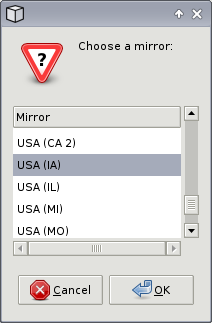
\includegraphics[width=2in,height=3in]{cran-mirror.png}
    \hspace{.5in}
    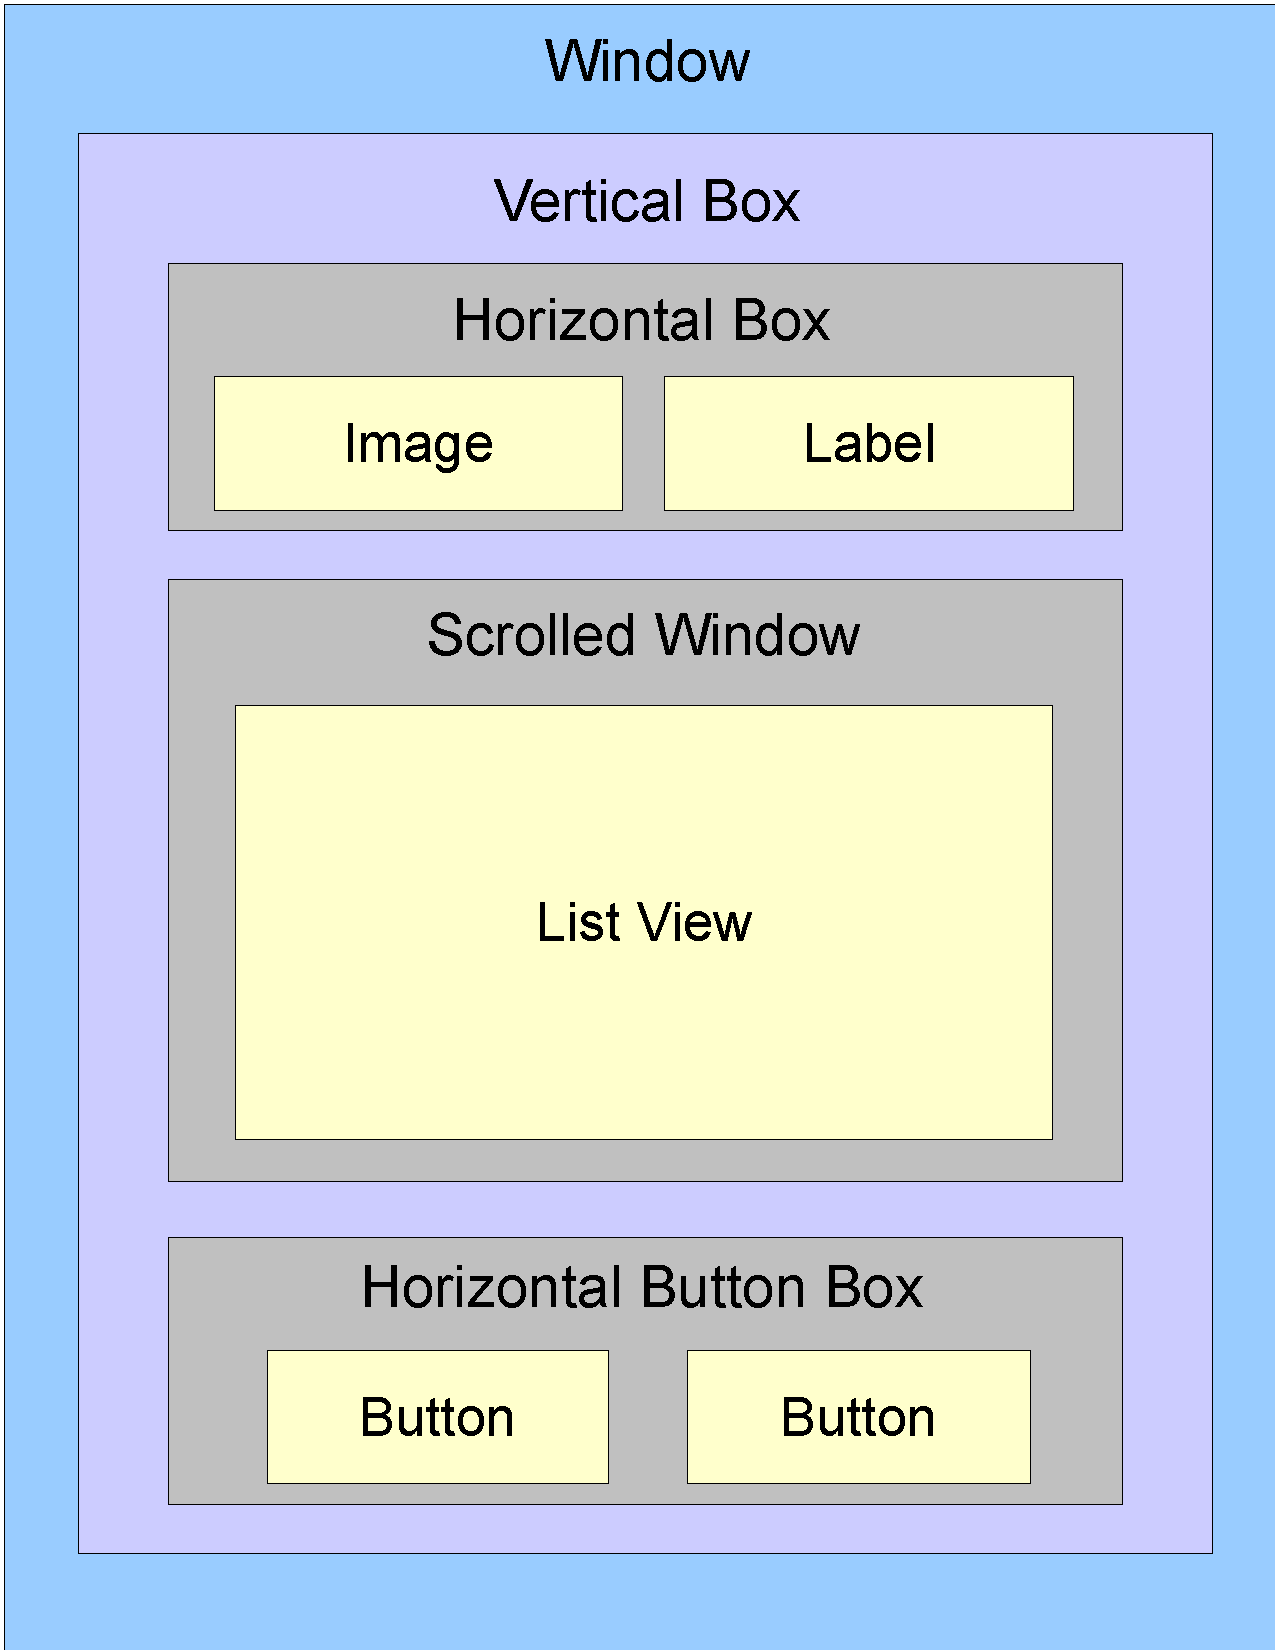
\includegraphics[width=2in,height=3in]{widget-hierarchy.pdf}
    \caption{\label{fig:cran-mirror}\label{fig:widget-hierarchy} A
dialog
      for selecting a CRAN mirror constructed using the \pkg{RGtk2}
package. The
      screenshot of the dialog is shown on the left. The user selects
a
      mirror from the list and clicks the \code{OK} button to confirm
the
      choice.  In the image on the right, each rectangle corresponds
to a
      widget in the GUI. The window is at the top-level, and each of
the
      other widgets is geometrically contained within its parent. Many
of
      the container widgets are invisible in the screenshot.}
  \end{center}
\end{figure}

% RGtk2
\pkg{RGtk2} is a GUI toolkit for \proglang{R} derived from the
\pkg{RGtk} package.
Like \pkg{RGtk}, \pkg{RGtk2} provides programmatic access to
\pkg{GTK+}, 
a cross-platform (Windows, Mac, and Linux) widget toolkit. 
% DTL: already cited \citep{GTK}.
The letters \emph{GTK} stand for the \emph{GIMP ToolKit}, with the
word \emph{GIMP} recording the origin of the library as part of the
GNU Image Manipulation Program. \pkg{GTK+} is written in \proglang{C},
which
facilitates access from languages like \proglang{R} that are also
implemented 
in \proglang{C}. It is licensed under the \emph{Lesser GNU Public
License} (LGPL).
%DTL:  meaning that \pkg{GTK+} does not force a specific license on
%the software that uses it.
% Yes it does. It forces the LGPL by definition
%which provides greater flexibility 
% and more wide-spread use 
%DTL2:  "more wide-spread" would need some verification and there are
%some who don't like the freedom the LGPL provides for commercial
%interests to use the code in proprietary systems. 
%than the regular GNU Public License (GPL).
%This contributes to its popularity.
%DTL2: again, this is debatable and needs evidence.
% I think it is unnecessary to make claims about popularity and
% flexibility as they are undefined terms and highly subjective. 
\pkg{GTK+} provides the same widgets on every platform, though it can be customized to emulate platform-specific look and feel. The original \pkg{RGtk} is bound to the previous generation of \pkg{GTK+}, version 1.2. \pkg{RGtk2} is based on \pkg{GTK+ 2.0}, the current generation. Henceforth, this paper will only refer to \pkg{RGtk2}, although many of the fundamental features of \pkg{RGtk2} are inherited from \pkg{RGtk}. The package is available from the Comprehensive \proglang{R} Archive Network (CRAN) at \url{http://CRAN.R-project.org/package=RGtk2}.

% outline
We continue with the fundamentals of the \pkg{GTK+} GUI and the
\pkg{RGtk2} package. This is followed by a tutorial, including
examples, on using \pkg{RGtk2} to construct basic to intermediate
GUIs. The paper then moves into a more technical domain, introducing
the advanced features of the interface, including the creation of new
types of widgets. We then present a technical description of the
design and generation of the interface, which is followed by a
discussion of more general binding issues.  Next, we compare
\pkg{RGtk2} to existing GUI toolkits in \proglang{R}.  We conclude by
mentioning some applications of \pkg{RGtk2} and explore directions for
future development.

\section{Fundamentals}

This section begins with an introduction to the basic widgets and
elements of the of the \pkg{GTK+} library.  We then turn our attention
to the \pkg{RGtk2} interface to \pkg{GTK+}, explaining how to
create and manipulate widgets and how to respond to user input. The
section concludes by introducing widget layout, the process of
determining the size and position of each widget on the screen.

% This section introduces the CRAN mirrors GUI as a goal, but 
% begins with the classic "Hello World" button-in-a-window GUI

\subsection[GTK+ widgets]{\pkg{GTK+} widgets}

\subsubsection{Widget type hierarchy}

%DTL:  Strange that we refer first to figure 2 and then figure 1.
% Why not put figure 1 and 2 side-by-side in a single figure and label
% them a) and b).
% Also, the part of the widget hierarchy in Figure 1 doesn't really
% relate to the GUI in figure 2.
%ML: I placed the CRAN mirror GUI and the widget hierarchy together.
% They now come before the class hierarchy.

%DTL2: Thanks. In my version, figure 1 is still the class hierarchy.

The left panel of Figure~\ref{fig:cran-mirror} shows a \pkg{GTK+} GUI
that allows the user to select a CRAN mirror for downloading
\proglang{R} packages.  This GUI is likely familiar to many
\proglang{R} users, since a similar interface is present in the
official Windows and Mac OS X \proglang{R} GUIs, among others.  There
are several different types of widgets in the CRAN mirrors GUI.  A
text label instructs the user to choose a mirror.  A list
control/widget contains the names of the available mirrors, and there
are buttons for confirming or canceling the choice.  The interface is
enclosed by another type of widget, a window.

All of these widget types have functionality in common. For example,
they are all drawn on the screen in a consistent style. To formalize
this relationship and to simplify implementation by sharing code
between widgets, \pkg{GTK+} defines an inheritance hierarchy for its
widget types, or classes. A small portion of the \pkg{GTK+} class
hierarchy is shown in Figure~\ref{fig:class-hierarchy}. For specifying
the hierarchy, \pkg{GTK+} relies on \pkg{GObject}, a \proglang{C}
library that implements a class-based, single-inheritance
object-oriented system.  Each type of \pkg{GTK+} widget is a
\pkg{GObject} class that inherits from the base \code{GtkWidget} class
which provides the general characteristics shared by all widget
classes, e.g., properties giving the location, color; methods for
hiding, showing and painting the widget. A \pkg{GObject} class
encapsulates behaviors that all instances of the class share.  Each
class has a single parent from which it inherits the behaviors of its
ancestors. A class can override some specific inherited behaviors.  A
more detailed and technical explanation of \pkg{GObject} is available
in Section~\ref{sec:primer}.

\begin{figure}[h!tbp]
\begin{center}
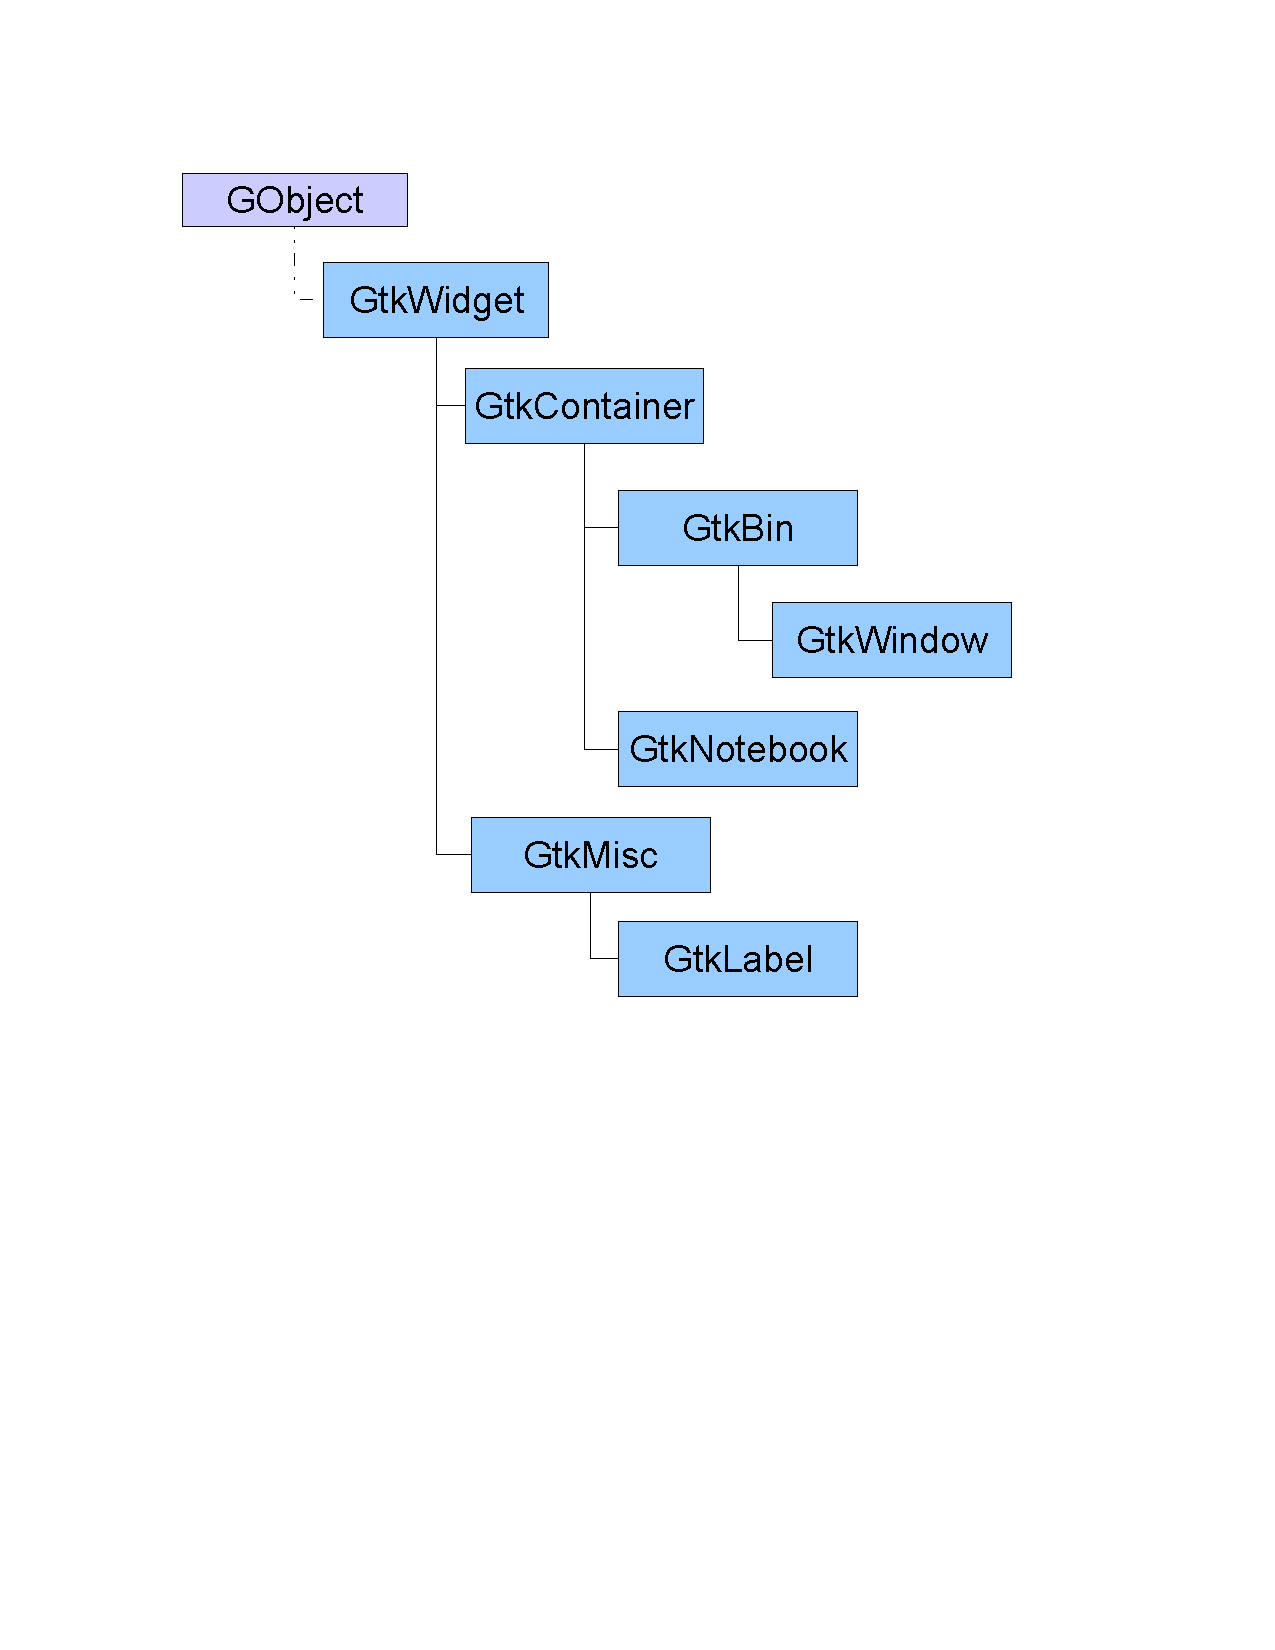
\includegraphics[width=3in]{class-hierarchy.pdf}
\caption{\label{fig:class-hierarchy}A small portion of the GTK+ class
hierarchy. 
All widgets are derived from the \code{GtkWidget} class, which is
derived, 
indirectly, from the \code{GObject} base class.}
\end{center}
\end{figure}

\subsubsection{Widget container hierarchy}

There is another tree hierarchy that is orthogonal to the class
inheritance hierarchy. This hierarchy involves widget instances rather
than widget classes. Each widget instance has a single parent instance
in which it is contained, except for a top-level window which has no
parent
and serves as the root of the tree. Child widgets are contained within
the rectangular region of their parents.
%DTL2:  can you explain what geometrically means in this context.
%MFL2: reworded
In Figure~\ref{fig:cran-mirror}, for
example, the label, list of mirrors, and buttons are all contained
within the top-level window, meaning that the window is the common
ancestor of the other widgets.  The right panel of Figure~\ref{fig:widget-hierarchy} shows, in a simplified way, the two
dimensional nesting of the widgets in the mirror selection
example. Widgets that can contain other widgets are called
\emph{containers} and their classes are derived from the
\code{GtkContainer} class. Windows and tabbed notebooks are examples
of containers.  Combining primitive widgets like labels and icons
within containers leads to more complex displays, such as menus,
tool bars and even buttons which contain labels to display the text. A
container is responsible for allocating its space to its
children. This process is called layout management and is described in
Section~\ref{sec:layout}.

\subsection[GTK+ widgets in R]{\pkg{GTK+} widgets in \proglang{R}}
\pkg{RGtk2} provides an Application Programming Interface (API) to the
\pkg{GTK+} 
library. A programmer uses an API to create an application based on
functions implemented
within a separate module. It is a contract that specifies in detail
the functionality available to a programmer without specifying how
that functionality is implemented. 
%DTL: I am not certain that continuing the Unwin & Hoffman definition
%of an interface helps as much here as saying that an API is like a
%contract that specifies in detail what is available to a programmer 
% but not how things are implemented.  It is a declaration rather than
% an interface.  I don't think identifying the module as a machine
% helps.
 
% ML: I added a sentence along the lines of it defining a contract. I
% would still argue, however, that an API is a user interface.
% DTL:  I don't disagree, but I don't think the analogy is very
% helpful
% in this particular case as it doesn't help to clarify things for the
% reader and certainly runs the risk of confusing the concept of a
% graphical user interface with programmer user interface.  So no
% disagreement on concept, just a choice of presentation.

% MFL2: I see what you mean. I guess I was only trying to relate APIs
% to GUIs, but that offers little benefit and is likely confusing


As with other user interfaces,
an API should be consistent and efficient to use. As an \proglang{R}
package,
\pkg{RGtk2} primarily aims to be consistent with \proglang{R}
conventions. This
means hiding aspects of the \pkg{GTK+} API that are foreign to
\proglang{R},
such as explicit memory management. A secondary concern is consistency 
with the underlying \pkg{GTK+} API. The developers of
\pkg{GTK+} have invested a significant amount of thought into its
design. Thus,
\pkg{RGtk2} endeavors to interface \proglang{R} to the virtual
entirety of \pkg{GTK+},
without leaving any gaps that may be unanticipated by the user. 
The only omissions are those that would violate consistency with
\proglang{R}. For example, functions related to explicit memory
management were excluded, as memory in \proglang{R} is managed by a
garbage collector. Array length parameters are also excluded, as the
length of a vector is always known in \proglang{R}.
%DTL: e.g.,  some examples
The \pkg{RGtk2} API has also been designed for ease/efficiency of use.
Towards this end, it specifies a default value for a function
parameter whenever sensible and uses a special object-oriented syntax,
as introduced by the \pkg{SJava} package \citep{sjava}.
%DTL: RGtk didn't introduce the special syntax. It was first
%introduced in the SJava package.

To demonstrate the basic syntax and features of the \pkg{RGtk2} API,
we will construct a simple ``Hello World'' GUI, shown in Figure~\ref{fig:hello-world}.

\begin{figure}[h!tbp]
\begin{center}
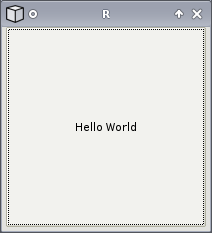
\includegraphics[width=2in]{hello-world.png}
\caption{\label{fig:hello-world}``Hello World'' in GTK+. 
A window containing a single button displaying a label with the text
\code{Hello World}.}
\end{center}
\end{figure}

We will gradually 
progress from this trivial GUI to the aforementioned CRAN mirrors GUI
and beyond.
The first step is to create a top-level window to contain our GUI.
Creating an instance of a \pkg{GTK+} widget requires calling a single
\proglang{R} 
function, known as a constructor. The constructor for a class has the
same name as the class, except the first character is lowercase. The
following statement constructs an instance of the
\code{GtkWindow} class:
\begin{Code}
window <- gtkWindow("toplevel", show = FALSE)
\end{Code}

The first argument to the constructor for \code{GtkWindow} corresponds
to the type of the top-level window. The set of possible window types
is specified by what in \proglang{C} is known as an
\emph{enumeration}. Since enumerations are foreign to \proglang{R},
\pkg{RGtk2}
accepts string representations of enumeration values, like
\code{"toplevel"}. For every \pkg{GTK+} enumeration, \pkg{RGtk2}
provides
an \proglang{R} vector that maps the nicknames to the underlying
numeric values.  In the above case, the vector is named
\code{GtkWindowType}. The expression \code{names(GtkWindowType)}
returns the names of the possible values of the \code{GtkWindowType}
enumeration, and the same applies to all other enumerations. It is
rarely necessary to explicitly use the
enumeration vectors; specifying the nickname will work in most cases,
including all method invocations and is preferable as it is easier for
human readers to comprehend. 

%DTL2:  it would be good to identify here (or elsewhere later in the
%article) how one can find the possible values for an enumeration
%type.  As it stands, the user must know the nickname. But she might
%want to see all the possible values in order to chose the relevant
%one.




The \code{show} argument is the last argument for every widget
constructor. It indicates whether the widget should be made visible
immediately after construction.  The default value of \code{show} is
\code{TRUE}. In this case we want to defer showing the window until
after we finish constructing our simple GUI.

%DTL: This next paragraph hangs out a little, i.e., it doesn't flow
%directly from the previous paragraphs but introduces a new concept
%and then we move on to another.  It is okay, but it would be nice to
%try to connect it a little more.
The next steps are to create a ``Hello World'' button and to place the
button in the window that we have already created. This depends on an
understanding of how of one programmatically manipulates widgets.
Each widget class defines an API consisting of methods, properties,
fields and signals. Methods are functions that take an instance of
their class as the first argument and are used to instruct the widget
to perform an action. Properties and fields store the public state of
a widget. Examples of properties include the title of a window, the
label on a button, and whether a widget has the keyboard focus.
%DTL: e.g., give some examples.
Signals are emitted as a result of events, such as user interaction
with a widget.
%DTL: signals can be omitted by programmatic actions also.
By attaching an \proglang{R} handler function to a widget's signal, we
can
perform an action in response to all user inputs that generate that
signal. We explain how one can interface \proglang{R} functions with
each of these in the following sections as we continue with our
``Hello World'' example.

\subsubsection{Invoking methods}

Methods are functions that operate on widgets inheriting from a
particular class.  The \pkg{RGtk2} function for each \pkg{GTK+} method
is named according to the \emph{classNameMethodName} pattern. For
example, to add a child to a container, we need to invoke the
\code{add} method on the \code{GtkContainer} class.  The corresponding
function name would be \code{gtkContainerAdd}.  However, this
introduces an inefficiency in that the user needs to remember the
class to which a method belongs. To circumvent this problem, we
introduce a syntax that is similar to that found in various
object-oriented languages. The widget variable is given first,
followed by the \code{\$} operator, then the method name and its
arguments. This syntax for calling \code{gtkContainerAdd} is
demonstrated below as we add a button with the label \code{Hello
World} to our window.  The third statement calls
\code{gtkWindowSetDefaultSize} to specify our desired size for the
window when it is first shown. The code for these method invocations
is below:
\begin{Code}
button <- gtkButton("Hello World")
window$add(button)
window$setDefaultSize(200, 200)
\end{Code}
Each method belongs to a separate
class, but the syntax frees the user from the need to remember the
exact classes and also saves some typing as 
the \code{\$} operator finds the most specific/appropriate method based on
the class inheritance of the widget.
Note that we use the lower case form of the first letter when using
the \code{\$} syntax, but the upper case form in the
\code{classNameMethodName} function name. The \code{\$} acts as a word
separator and we use lower case at the beginning of new words.



\subsubsection{Accessing properties and fields}

Properties are self-describing 
%DTL2: explain what self-describing means here, i.e., provide run-time
%information about their type.
% However, perhaps mentioning this here is too technical and somewhat
% irrelevant to the user looking for an overview at this point.
elements that store the state of an aspect of a widget.  Examples of
properties include the title of a window, whether a checkbox is
checked, and the length in characters of a text entry box. The
%DTL2:  Is this [ or [[. Perhaps [[ but fine to leave as is. Just need
%to be consistent. The dialog example on page 13 seems to use
%dialog[["vbox"]]
% MFL2: The '[' gets properties, the '[[' gets fields, as far as the
%paper is concerned anyway. In the code, they may be interchangeable.
\proglang{R} subset function \code{[} may be used to get the value of
a widget property by name.  Below we access the value of the
\code{visible} property of our window:
\begin{CodeChunk}
\begin{CodeInput}
R> window["visible"]
\end{CodeInput}
\begin{CodeOutput}
[1] FALSE
\end{CodeOutput}
\end{CodeChunk}
We find that the value is
\code{FALSE}, since we specified it not to be shown at construction
and have not made it visible since then.

\pkg{GTK+} properties may be set, given that they are writable, using
the regular \proglang{R} assignment operator (\code{<-} or \code{=}).
This is
actually implemented via the \code{[<-} method for \pkg{GTK+} widgets
in \pkg{RGtk2}. The example below makes the window created above
visible, using both property-setting methods,
the second corresponding to a call to \code{gtkWidgetShow}, which is
more conventional:
\begin{Code}
window["visible"] <- TRUE 
window$show()
\end{Code}

For convenience, one might desire to set multiple properties with a
single statement.
This is possible using the \code{gObjectSet} method, which behaves
similarly
to the \proglang{R} \code{options} function, in that the argument name
indicates
the property to set to the argument value. 
%DTL: Perhaps make note that this is gObjectSet and not gtkObjectSet.
In the single statement below, we 
set the window icon to the \pkg{RGtk} logo image and set the title to
\code{"Hello World 1.0"}:
\begin{Code}
image <- gdkPixbuf(filename = imagefile("rgtk-logo.gif"))[[1]]
window$set(icon = image, title = "Hello World 1.0")
\end{Code}
The \code{imagefile} function retrieves an image from the \pkg{RGtk2}
installation.
\code{gdkPixbuf} returns a list, where the first element is a
\code{GdkPixbuf}, an image object,
and the second is a description of an error encountered when reading
the file
or \code{NULL} if the operation was successful. Here we assume that
there is no error.

In rare cases, it is necessary to access a field in the widget data
structure.
Fields are different from properties in several ways. Most
importantly, it is
never possible to set the value of a field. The user can retrieve the
value of
a field using the \code{[[} function. For example, now that our window
has been shown, it has been allocated a rectangle on the screen. This
is stored
in the \code{allocation} field of \code{GtkWidget}. It returns a list 
representing a \code{GtkAllocation} with elements \code{x}, \code{y},
\code{width} and \code{height}, as in the code segment below:
%DTL:  Why doesn't this have a class such as GdkRectangle. We are
%losing information about the object which is available from the
%property.

% ML: This appears to be a bug. It seems that some of the older 
% conversion routines that I implemented manually do not set the class
% attribute. Weird how I never noticed that.
%DTL2: I know that feeling!
\begin{CodeChunk}
\begin{CodeInput}
R> window[["allocation"]]
\end{CodeInput}
\begin{CodeOutput}
$x
[1] 0

$y
[1] 0

$width
[1] 200

$height
[1] 200

attr(,"class")
[1] "GtkAllocation"
\end{CodeOutput}
\end{CodeChunk}
%DTL2:  class of the object should be RGdkRectangle (or whatever)


\subsubsection{Handling signals/events}

Once a GUI is displayed on the screen, the user is generally free to
interact with it. Examples of user actions include clicking on
buttons, dragging a slider and typing text into an entry box.  In the
CRAN mirrors example, possible user actions include selecting a mirror
in the list, clicking the \code{OK} or \code{Cancel} buttons and
pressing a
keyboard shortcut, such as \texttt{Alt-O} for \code{OK}.  An
application
may wish to respond in a certain way to one or more of such actions.
The CRAN mirrors application, for example, should respond to an
\code{OK}
response by saving the chosen mirror in the session options.

So far, we have created and manipulated widgets by calling a list of
procedures in a fixed order. This is convenient as long as the
application is ignoring the user. Listening to the user would require
a loop which continuously checks for user input.  It is not desirable
to implement such a loop for every application, so \pkg{GTK+} provides
one for all GUI applications to use within the same \proglang{R}
session. When an
application initializes the \pkg{GTK+} event processing loop, there is
an \emph{inversion of control}. The application no longer has primary
control of its flow; instead, \pkg{GTK+} asynchronously informs the
application of events through the invocation of functions provided by
the application to handle a specific type of event. These handlers are
known as \emph{callbacks}, because \pkg{GTK+} is calling back into the
application.

\pkg{GTK+} widgets represent event types as signals. One or more
callbacks can be connected to a signal for each widget instance. When
the event corresponding to the signal occurs, the signal is emitted
and the callbacks are executed in an order depending on how they were
connected. In order to execute \proglang{R} code in response to a user
action on a widget, we connect an \proglang{R} function to the
appropriate signal on the widget.  The \code{gSignalConnect} function
performs this connection. The following code will make our ``Hello
World'' example from above more interactive:  
\begin{Code}
gSignalConnect(button, "clicked", 
               function(widget) print("Hello world!"))
\end{Code}
The call to
\code{gSignalConnect} will cause \code{"Hello world!"} to be printed
upon emission of the \code{clicked} signal from the button in our
window.  The
\code{clicked} signal is emitted when the user clicks the button with
a pointer device or activates the button with a keyboard shortcut.

\subsubsection{Widget documentation}

Documentation for widgets is available using the conventional
\proglang{R} 
\code{help} command. It is derived from the documentation of
\pkg{GTK+} itself.
To see the methods, properties, fields, and signals available
for a particular class, the user should access the help topic matching
the class name.
For example, to read the documentation on \code{GtkWindow} we enter:
\begin{Code}
help(GtkWindow)
\end{Code}

Similarly, the detailed help for a specific method is stored under the
full name of the function. For example, to learn about the \code{add}
method on \code{GtkContainer}, we enter:
\begin{Code}
help(gtkContainerAdd)
\end{Code}
%DTL2:  We should also be able to do something along the lines of 
%   help(w$add)
% where w is a container widget and find the relevant method.  The
% operator ? in tends to work this way.

\subsection{Widget layout}\label{sec:layout}
%DTL2:  Take a read over this and see if it is clear and comprehensive
%for you. I think it is a little unclear and perhaps a few sentences
%would aid greatly. Not sure where at this point. Sorry !


In our ``Hello World'' example, we added only a single widget, a
button, to the  top-level window. In contrast, the CRAN mirrors window
contains multiple widgets, which introduces the problem of
appropriately allocating the space in a window to each of its
descendents in the container hierarchy. This problem is often called
\emph{layout management}. Laying out a GUI requires specifying the
position and size of each widget below the top-level window. The
simplest type of layout management is static; the position and size of
each widget are fixed to specific values. This is possible
with \pkg{GTK+}, but it often yields undesirable results. A GUI is
interactive and changes in response to user input. The quality of a
fixed layout tends to decrease with certain events, such as the user
resizing the window, a widget changing its size requirement, or the
application adding or removing widgets. For this reason, most layout
management is dynamic.

In \pkg{GTK+}, containers are responsible for the layout of their
children. The right panel in Figure~\ref{fig:widget-hierarchy} shows
how the nesting of layout containers results in the CRAN mirrors GUI
shown in Figure~\ref{fig:cran-mirror}. The example employs several
important types of \pkg{GTK+} layout containers. 

First, there is the
top-level \code{GtkWindow} that is derived from \code{GtkBin}, which
in turn derives from \code{GtkContainer}.  A \code{GtkBin} holds only
a single child, and \code{GtkWindow} simply fills all of its allocated
space with its child. 

The most commonly used container for holding
multiple children is the general \code{GtkBox} class, which stacks its
children in a specified order and in a single direction, vertical or
horizontal. The children of a \code{GtkBox} always fill the space
allocated to the box in the direction orthogonal to that of the
stacking, e.g., fill the available width when stacked vertically on top
of each other. 

The \code{GtkBox} class is abstract (or virtual), meaning
that one cannot create instances of it. Instead, we instantiate one of
its non-abstract subclassses.  For example, in the CRAN mirror GUI, a
vertical box, \code{GtkVBox}, stacks the label above the list, and a
horizontal button box, \code{GtkHButtonBox}, arranges the two
buttons. \code{GtkVBox} and its horizontal analog \code{GtkHBox} are
general
%DTL2: I think this should be general rather than generic.  At least,
%generic in the technical sense and since R uses the word "generic"
% in a specific manner, it is probably best to avoid this.
layout containers, while the button boxes \code{GtkVButtonBox}
and \code{GtkHButtonBox} offer facilities specific to the layout of
sets of buttons.
%DTL: perhaps mention that GtkBox is a virtual class of which we never
%create instances and we use the derived classes GtkHBox and GtkVBox.

Here we will explain and demonstrate the use of \code{GtkHBox}, the
general horizontal box layout container. \code{GtkVBox} can be used
exactly the same way; only the direction of stacking is different.
Figure~\ref{fig:packing} illustrates a sampling of the possible
layouts that are possible with a \code{GtkHBox}.

%DTL: It would be good to number the rows so that people can easily
%connect the descriptions in the text to the particular row.
\begin{figure}[h!tbp]
\begin{center}
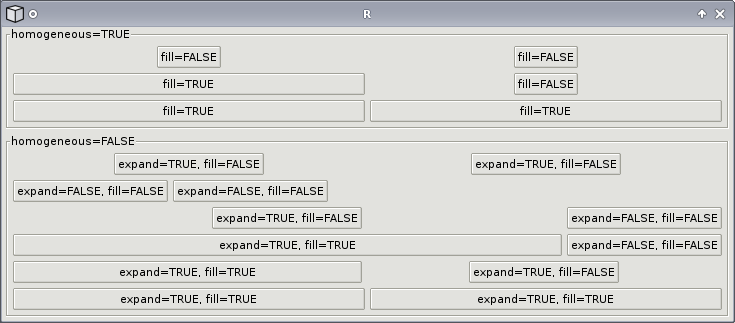
\includegraphics{packing.png}
\caption{\label{fig:packing}A screenshot demonstrating the effect of
packing two
buttons into \code{GtkHBox} instances using the \code{gtkBoxPackStart}
method 
with different combinations of the \code{expand} and \code{fill}
settings. 
The effect of the \code{homogeneous} spacing setting on the
\code{GtkHBox} is 
also shown.}
\end{center}
\end{figure}

The code for some of these layouts is presented here. We begin by
creating a \code{GtkHBox} widget. We pass \code{TRUE} for the
first parameter, \code{homogeneous}. This means that the horizontal
allocation of the box will be evenly distributed between the children. 
The second parameter directs the box to leave 5 pixels of space
between each child.  The following code constructs the \code{GtkHBox}:
\begin{Code}
box <- gtkHBox(TRUE, 5)
\end{Code}
The equal distribution of available space is strictly enforced; the
minimum size requirement of a homogeneous box is set such that the box
always satisfies this assertion, as well as the minimum size
requirements of its children.

The \code{gtkBoxPackStart} and \code{gtkBoxPackEnd} methods pack a
widget into a box with left and right justification (top and
bottom for a \code{GtkVBox}), respectively. For this explanation, we
restrict ourselves to \code{gtkBoxPackStart}, since
\code{gtkBoxPackEnd} works the same except for the
%DTL: direction or justification?
justification. Below, we pack two buttons, \code{button\_a} and
\code{button\_b} using left justification:
\begin{Code}
button_a <- gtkButton("Button A")
button_b <- gtkButton("Button B")
box$packStart(button_a, fill = FALSE)
box$packStart(button_b, fill = FALSE)
\end{Code}
First, \code{button\_a} is packed against the left side of the box,
and then we pack \code{button\_b} against the right side of
\code{button\_a}.
The space distribution is homogeneous, but
the extra space for each widget is not filled. This results in the
first row in Figure~\ref{fig:packing}.

Making the space available to a child does not mean that the
child will fill it. That depends on the minimum size requirement of
the child, as well as the value of the \code{fill} parameter passed to
\code{gtkBoxPackStart}. When a widget is packed with the \code{fill}
parameter set to \code{TRUE}, the widget is sized to consume the
available space. This results in rows~$2$ and $3$ in Figure~\ref{fig:packing}.

%DTL2: This is the confusing part.

In many cases, it is desirable to give children unequal amounts of
available space, as in rows~4--9 in Figure~\ref{fig:packing}. This is
evident in the CRAN mirrors dialog, where the mirror list is given
more space than the \code{Please choose a mirror} label. To create an
inhomogeneously spaced \code{GtkHBox}, we pass
\code{FALSE} as the first argument to the constructor, as in the
following code:
\begin{Code}
box <- gtkHBox(FALSE, 5)
\end{Code}

An inhomongeneous layout is freed of the restriction that all widgets
must be given the same amount of available space; it only needs to
ensure that each child has enough space to meet its minimum size
requirement. After satisfying this constraint, a box is often left
with extra space. The programmer may control the distribution of this
extra space through the \code{expand} parameter to
\code{gtkBoxPackStart}.  When a widget is packed with \code{expand}
set to \code{TRUE}, we will call the widget an \emph{expanding}
widget. All expanding widgets in a box are given an equal portion of
the entirety of the extra space. If no widgets in a box are expanding,
as in row~5 of Figure~\ref{fig:packing}, the extra space is left
undistributed. It is common to mix expanding and non-expanding widgets
in the same box. For example, in the CRAN mirrors dialog, the box
first ensures that the mirror list and the label above it are given
enough space to satisfy their minimum requirement. Then, since the
mirror list is expanding, all of the extra space is made available to
it, while the label is left only with its minimum requirement (i.e.,
enough space to show its text).
%DTL2: against is a strange term here. I don't understand it properly.
% So either it needs clarification or let's chose another word, e.g.,
% expands, "consuming the space given to the other children".
%MFL2: reworded this
% Is this really its "available space". There seems to be an
% imprecision here that will confuse people.
%MFL2: Available space is space the widget *could*, consome whether it
% does depends on its space requirements and the fill parameter.
Another example is given below, where \code{button\_a} is expanding,
while \code{button\_b} is not:
\begin{Code}
box$packStart(button_a, expand = TRUE, fill = FALSE)
box$packStart(button_b, expand = FALSE, fill = FALSE)
\end{Code}
The result is shown in row~6 of Figure~\ref{fig:packing}. 
The figure contains several other permutations of the
\code{homogeneous}, \code{expand} and \code{fill} settings.

\pkg{GTK+} contains many types of layout containers besides boxes,
including 
a grid layout (\code{GtkTable}), a user-adjustable split pane
(\code{GtkHPaned}
and \code{GtkVPaned}), and a tabbed notebook (\code{GtkNotebook}).
More types of
layout containers will be demonstrated later in the tutorial.


%DTL2:  To complete the overview, it would seem that there should be 
% a description of callbacks at this point giving the basics about
% how they are connected, the number and types of arguments they will
%be called with.

%MFL: Isn't this covered sufficiently in the signals section above?

\section{Basic GUI construction}

% a relatively simple first gui: dialogs (just a message, multiple
%buttons)
% giving the user more choices: check button, radio buttons, combo box
% in dialogs
% CRAN mirrors example (list dialog)
% alpha-slider (microarray) example
%   (approximiately) continuous choices: slider, (spin button)
%   displaying information as graphics: cairoDevice, mention
%GtkDrawingArea
% spreadsheet app: 
%   advanced choosers: files, mention colors, fonts
%   displaying tabular information: tree view
%   arbitrary text input: text entry (completion)
%   advanced containers: 
%     space saving / hiding: menu bar, tool bar, scrolled window,
% notebook, (expander)
%     (letting the user decide: pane)
%   displaying status: status bar (progressbar)
%   assisting the user: tooltips, (wizard)
% moving data around: dnd, clipboard

Thus far, we have reviewed the fundamentals of \pkg{GTK+}, working
with
\pkg{GTK+} widgets from \proglang{R}, and widget layout management. In
this
section, we will build on this foundation to create some basic but
potentially
useful GUIs. 

Constructing a GUI may be conceptually divided into two basic steps.
First, one must create the individual widgets, specify their
properties,
and organize them into containers. This defines the physical aspect
of the GUI: the appearance of the widgets and their spatial
organization.
The second step defines the behavior or the logical aspect of the
interface. It involves registering handlers for signals that are
emitted
by the widgets, for example in response to a user pressing a button.
The signal handlers encapsulate the logic beneath the interface. In
this
section, we will demonstrate these two steps and show how their
integration
results in functional GUIs.

\subsection{A dialog with the user}\label{sec:dialog-example}

A user interface is the conduit for a conversation between the machine
and the user. This conversation may be broken down into a series of
exchanges called \emph{dialogs}. An application often needs to make a
specific request for user input, such as the desired CRAN mirror. This
type of dialog is initiated by the machine posing a question to the
user. The machine then waits for the user to respond. Usually, the
application is unable to continue until receiving the user response,
so the rest of the GUI is blocked until the dialog is concluded. This
is called a \emph{modal} dialog.  A dialog is described as
\emph{non-modal} when the user can continue to perform other tasks
even when the dialog is displayed.

\begin{figure}[tbp]
  \begin{center}
    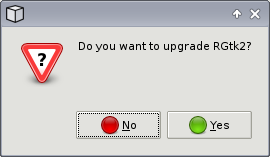
\includegraphics[width=3in]{upgrade-dialog.png}
    \caption{\label{fig:upgrade-dialog}A screenshot of a message
dialog
      requesting a 
      ``Yes'' or ``No'' response from the user.}
  \end{center}
\end{figure}

\pkg{GTK+} explicitly supports modal and non-modal requests for user
input with a dialog widget, a top-level window that emits the
\code{response} signal when the user has responded to the query. All
dialogs in \pkg{GTK+} are derived from the \code{GtkDialog} class. The
CRAN mirrors GUI is an instance of \code{GtkDialog}. In the simpler
example below,
%DTL2:  can we label this with a formal paragraph title so that it is
%more obvious to what this refers.
%MFL: I'm a little confused about what you mean here...
we will create a dialog that asks whether the user wants to upgrade
the \pkg{RGtk2} package installed on the system. Although we could
build such a dialog using \code{GtkDialog} directly,
\code{GtkMessageDialog}, an extension of \code{GtkDialog}, reduces the
amount of necessary code
%DTL2: for whom - the user or programmer. It is presumably the
%programmer so easier to say that it is less code for the programmer
% and the is more than just less typing, but also less code to
% maintain, fewer bugs, etc.
for queries that can be expressed with a textual message and a
set of buttons for the response. The dialog is constructed with a
single function call:
\begin{Code}
main_application_window <- NULL
dialog <- gtkMessageDialog(main_application_window,  
                           "destroy-with-parent", "question",
                           "yes-no", "Do you want to upgrade RGtk2?")
\end{Code}
In the above invocation, the first parameter of the call to 
\code{gtkMessageDialog} indicates the parent window for the dialog. It
is assumed that the main window of the application is stored as
\code{main\_application\_window}. The second parameter indicates that
the dialog should be destroyed when its parent, the main window, is
destroyed.  The next parameter specifies that this is a
\emph{question} dialog, which causes the dialog to display a question
mark icon to the left of the text.  The predefined set of buttons, in
this case consisting of \code{Yes} and \code{No}, is given by the next
parameter. The final parameter specifies the text of the message.  The
resulting dialog is shown in Figure~\ref{fig:upgrade-dialog}.

It is desirable for this dialog to be \emph{modal}, meaning that user
interaction
%DTL2:  "focus" is a somewhat technical term here, so either use
%another or explain the concept.
is restricted to the dialog window until the user responds to the
question. By invoking the \code{gtkDialogRun} function, the dialog
becomes modal and execution is blocked until the user gives a
response, which is returned from the function. The following code
demonstrates the use of \code{gtkDialogRun}:
\begin{Code}
if (dialog$run() == GtkResponseType["yes"])
 install.packages("RGtk2")
dialog$destroy()
\end{Code}
If the user answered
``Yes'', our callback will install the latest version of the
\pkg{RGtk2} package. The call to \code{gtkWidgetDestroy} closes the
dialog window and renders it unusable, i.e., if the object is used in
subsequent computations, an error will be raised, because the dialog
widget is no longer valid.

The reference to \code{GtkResponseType} above is one of the rare cases
in which it is necessary to access an enumeration vector to retrieve
the numeric value for a nickname. The reason for this is that
\code{gtkDialogGetResponse} returns a plain numeric value to avoid an
unnecessary restriction on the number of possible response types from
a dialog. This allows programmers to introduce response types that do
not exist within the \code{GtkResponseType} enumeration.
%DTL2:  slightly confusing. Can you elaborate to say what this means
%in practice (i.e., that others can introduce additional return values)
In this case, it is known from the documentation of
%DTL2: how and can we automate this so that the relevant coversion is
%performed.
%MFL: it's difficult to automate, because we would have to assume that
% the return value is a GtkResponseType even though it is not
% contracted to be such by gtkDialogGetResponse. We could return a
% special type that when compared for equality with a string value
% would try to match a value in GtkResponseType... but I like to
% stay consistent with the GTK+ API when possible - it's a trade-off..
\code{GtkMessageDialog} that the value corresponding to the user
clicking the \code{Yes} button will equal the \code{yes} value in
\code{GtkResponseType}.

\subsection{Giving the user more options}
% toggle button, radio buttons, combo box

%DTL2:  Nice example to work through the different widgets.

Applications often need to ask questions for which a simple ``Yes'' or
``No'' answer does not suffice. As the number of possible responses to
a query increases, enumerating every response with a button would
place a burden on the user with a lengthy sequence of binary
questions.  It is easy to make a mistake when choosing one response
from many and hard to go back to correct such errors. An interface
should be forgiving and allow the user to confirm the choice before
proceeding.  This is how the CRAN mirrors dialog behaves: if the user
accidentally chooses a mirror on the other side of the world, the user
can correct the choice before clicking the \code{OK} button and
starting the installation process. This relates to the common need for
a program to issue a set of queries to the user. Separating each query
into its own dialog of buttons may unnecessarily force the user to
answer the questions in a fixed, linear order and may not be very
forgiving. It would also leave the user without a sense of context. If
there were many actions and choices available to the user, a
dialog-based interface would be tedious to use, requiring the user to
click through dialog after dialog. Instead, a less assertive,
non-linear interface is desired. In the examples below, we demonstrate
widgets that present options in a passive way, meaning that there is
usually no significant, immediate consequence to user interaction with
the widget and the user has to conclude the interaction by clicking
either the \code{OK} or \code{Cancel} button.

\begin{figure}[tbp]
  \begin{center}
    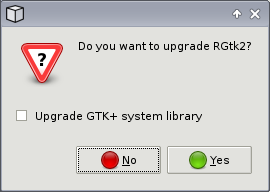
\includegraphics[width=3in]{checkbox-dialog.png}
    \caption{\label{fig:checkbox-dialog}A screenshot of a message
dialog
      with a 
      check box for requesting additional input on top of the
      original dialog in Figure~\ref{fig:upgrade-dialog}.}
  \end{center}
\end{figure}

The simplest user-level choice is binary and is usually represented in
a passive way via a checkbox with a checked/unchecked or  on/off 
state. In \pkg{GTK+}, the checkbox class is the
\code{GtkCheckButton}. We may wish to extend our dialog confirming the
upgrade of \pkg{RGtk2} to include the option of also upgrading the
underlying \pkg{GTK+} \proglang{C} library. In the snippet below, we
achieve this by adding a
check button to the dialog.  The area above the buttons in the
\code{GtkDialog} is contained within a \code{GtkVBox}, which is stored
as a field named \code{vbox} in the dialog object. Figure~\ref{fig:checkbox-dialog} shows
our custom checkbox dialog and the following code is how to create it:
\begin{Code}
dialog <- gtkMessageDialog(main_application_window,
                           "destroy-with-parent", "question",
                           "yes-no", "Do you want to upgrade RGtk2?")
check <- gtkCheckButton("Upgrade GTK+ system library")
dialog[["vbox"]]$add(check)
\end{Code}
%DTL2:  Is this a property (or actually a field as originally in the
%text) and do we need [[ or [ as just [ is used earlier in the
%document.

\begin{figure}[tbp]
  \begin{center}
    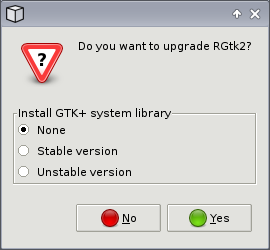
\includegraphics[width=3in]{radio-dialog.png}
    \caption{\label{fig:radio-dialog}A screenshot of a message dialog       with a set of radio buttons on top of the base dialog shown in       Figure~\ref{fig:upgrade-dialog}.}
  \end{center}
\end{figure}

Let us now suppose that we would like to give the user the additional
option of installing a development (experimental) version of
\pkg{GTK+}.  When an option has several choices, a check button is no
longer adequate. A simple approach is to create a set of toggle
buttons where only one button may be active at once. The buttons in
this set are known as \emph{radio buttons}, corresponding to the
pre-programed channel selection buttons on old-style radios.  Below,
we create a new dialog that asks the user to specify the version of
\pkg{GTK+} \proglang{C} libraries to install, if any: 
\begin{Code}
dialog <- gtkMessageDialog(main_application_window,
                           "destroy-with-parent", "question",
                           "yes-no", "Do you want to upgrade RGtk2?")
choices <- c("None", "Stable version", "Unstable version")
radio_buttons <- NULL
vbox <- gtkVBox(FALSE, 0)
for (choice in choices) {
  button <- gtkRadioButton(radio_buttons, choice)
  vbox$add(button)
  radio_buttons <- c(radio_buttons, button)
}
\end{Code}
When each radio button is created, it
needs to be given the existing collection of buttons already in the
group. For creating the first button, \code{NULL} should be passed as
the group.  Each button is added to a vertical box.

A group of radio buttons are often graphically enclosed by a drawn
border with a text label indicating the purpose of the buttons. This
widget is a container called \code{GtkFrame} and is generally used for
graphically grouping widgets that are logically related. The code
below adds the box containing the radio buttons to a newly created
frame:
\begin{Code}
frame <- gtkFrame("Install GTK+ system library")
frame$add(vbox)
dialog[["vbox"]]$add(frame)
\end{Code}
The final result is shown in Figure~\ref{fig:radio-dialog}.

\begin{figure}[tbp]
  \begin{center}
    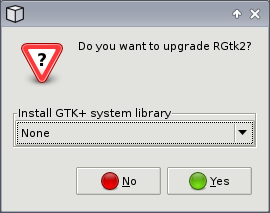
\includegraphics[width=3in]{combo-dialog.png}
    \caption{\label{fig:combo-dialog}A screenshot of a message dialog
with
      a 
      combobox for selecting an option from a drop-down menu before
      responding to
      the dialog.}
  \end{center}
\end{figure}

Now we would like to go a step further and allow the user to choose
the exact version of \pkg{GTK+} to install, as \pkg{RGtk2} is source
compatible with any version from $2.8.0$ onwards. As the number of
options increases, however, radio buttons tend to consume too much
space on the screen. In this case, a label displaying the current
selection with a drop down menu allowing for selecting from a list of
alternatives may be appropriate.  This is known as a
\code{GtkComboBox} in \pkg{GTK+}. The following snippet illustrates
its use. Each call to \code{gtkComboBoxAppendText} adds a text item to
the drop-down menu. The call to \code{gtkComboBoxSetActive} makes the
first item ($0$ due to zero-based counting in \proglang{C}) the
currently selected
one. Figure~\ref{fig:combo-dialog} shows the result and below is the
corresponding code:
\begin{Code}
dialog <- gtkMessageDialog(main_application_window,
                           "destroy-with-parent", "question",
                           "yes-no", "Do you want to upgrade RGtk2?")
choices <- c("None", "GTK+ 2.8.x", "GTK+ 2.10.x", "GTK+ 2.12.x")
combo <- gtkComboBoxNewText()
combo$show()
for (choice in choices) 
  combo$appendText(choice)

combo$setActive(0)
frame <- gtkFrame("Install GTK+ system library")
frame$add(combo)
dialog[["vbox"]]$add(frame)
\end{Code}

\subsection{The CRAN mirrors dialog}

Having demonstrated the creation some basic dialogs, we are now
prepared to construct the CRAN mirror selection dialog, shown in
Figure~\ref{fig:cran-mirror}.  Given the large number of CRAN mirrors,
one strategy would be to borrow the combobox dialog created above;
however, there may be a better alternative. Since there is no
reasonable default CRAN mirror, the user always needs to pick a
mirror. Packing the mirrors into a combo box would only force the user
to make an extra click.  Instead, we want to display a reasonable
number of CRAN mirrors immediately after the dialog is opened. It may
not be possible to display every mirror at once on the screen, but, as
seen in the screenshot, we can embed the list in a scrolled box, so
that only one part of the list is visible at a given time.

We begin with the construction of the dialog window, as below:
\begin{Code}
dialog <- gtkMessageDialog(NULL, 0, "question", "ok-cancel", 
                            "Choose a mirror:", show = FALSE)
\end{Code}
For this dialog,
we assume that there is no main application window (see Section~\ref{sec:spreadsheet-example}) to serve as the
parent. 
% DTL: The concept of an application window needs more explanation.
% It is defined in section 4 (Sample Application).
Instead, we pass \code{NULL} for the parent and \code{0} 
% DTL2:  What does 0 correspond to, i.e., what is the name for the
% enumerated constant.  It is not good practice to see literals in the
% code, especially for pedagogical purposes.
% MFL: This is a strange case - there is no name for 0 in the 
%GtkDialogFlags enumeration. It's the same for all "flags" in GTK+.
for the second argument rather than \code{"destroy-with-parent"}. We
use the literal \code{0} here instead of a value name, because
\code{GtkDialogFlags}, like all flag enumerations in \pkg{GTK+}, lacks
a value for $0$.

Next, we create a list for holding the mirror names using the
\code{GtkTreeView}
widget (so named because the rows in the list may be organized
hierarchically, but we will not discuss this feature). 
%DTL2: How does this correspond to R?  This might be going into too
%much generality here at the expense of confusion as the data
%structure is very simple - a vector and we are talking about
%hierarchical structure for which there is no counterpart in R and
%arbitrary number of ways to do this in C, so vague.  So I
%would leave this out, perhaps put the ability to deal with
%hierarchical data in a footnote.
% MFL: the intent was only to explain why we are using a widget named
% GtkTreeView when we are displaying a list.
The \pkg{RGtk2} package provides a facility for creating a tabular
data structure based on an \proglang{R} \code{data.frame},
called \code{RGtkDataFrame}. \code{RGtkDataFrame} is an extension of
\code{GtkTreeModel}, which is the data structure viewed by
\code{GtkTreeView}. Below, we create an \code{RGtkDataFrame} for our
list of CRAN mirrors and construct a \code{GtkTreeView} based on it:
\begin{Code}
mirrors <- read.csv(file.path(R.home("doc"), "CRAN_mirrors.csv"),
                     as.is = TRUE)
model <- rGtkDataFrame(mirrors)
view <- gtkTreeView(model)
view$getSelection()$setMode("browse")
\end{Code}
The final line configures the \code{GtkTreeView} so that exactly one
item is always selected in the view. This prevents the user from
providing invalid input (i.e., a multiple or empty selection). 
%DTL: This next bit is very detailed and specific relative to all the
%text in the document up until this point.
%ML: I included this explanation, because the GtkTreeView is very 
%complex. To really understand what is going on, even when just
%creating a simple list, one needs a complete explanation.

%DTL2: I still think this is less tangible and abstract than the
%reader will be able to master. So how about show the code first and
%then present this explanation later.
%
%  Also if something is "very complex", then it probably needs to be
% simplified
% and that is what RGtkDataFrame does. There is not much need to go
% into how it simplifies GtkTreeView, but just that it does simplify
% something more general and flexible which we don't need.  So I think
% we could  remove much of this and improve the readability and state
% that the RGtkDataFrame that you added to RGtk2 makes things simpler
% to use
% by building a higher-level interface to low-level a Gtk+ widget.
% So the explanation of the GktTreeView is actually not necessary
% because of your work.
%

%MFL: actually, the RGtkDataFrame only simplifies the data model -
% GtkTreeView is still quite complicated. Simplifying the creation
% of GtkTreeView would require only a single convenience function,
% implemented entirely in R. The gWidgets package provides this.
% RGtkDataFrame is more generally useful and is native code 
% (mostly for performance), so it remains part of RGtk2.
% I've tried to make the explanation less detailed though.

Initially, the tree view does not contain any columns. We need to
create a \code{GtkTreeViewColumn} to list the mirror names, and we do
so with the following code:
\begin{Code}
column <- gtkTreeViewColumn("Mirror", gtkCellRendererText(), text = 0)
view$appendColumn(column)
\end{Code}
The first parameter to \code{gtkTreeViewColumn} specifies the title of
the new column. Since we are displaying text (the names of the
mirrors) in the column, we pass an instance of
\code{GtkCellRendererText} which draws the values in our
\code{data.frame} as text in the \code{GtkTreeView}. The parameter
named \code{text} specifies that the first column of the
\code{data.frame} contains the values to draw as text. Note that the
index is zero-based (for historical reasons).
%DTL2:  This should be 1-based in R.
%MFL: we can consider this on the TODO list 
% - it would certainly break compatibility with existing work

Given the large number of CRAN mirrors, the list would take up
excessive space
if not embedded into a scrolled window. \code{GtkScrolledWindow} is a
container 
widget that provides a scrolled view of its child when the child
requests more
space than is available. In the following code, we add the tree view
to a \code{GtkScrolledWindow} 
instance that requests a minimum vertical size sufficient for showing
several mirrors at once:
\begin{Code}
scrolled_window <- gtkScrolledWindow()
scrolled_window$setSizeRequest(-1, 150)
scrolled_window$add(view)
\end{Code}
%DTL2:  Mention the units (pixels) for the 150
The size of \code{scrolled\_window} is set using
\code{gtkWidgetSetSizeRequest}, which takes values in pixel units.

It only remains to add the scrolled window to the dialog, run the
dialog, and set the selected CRAN mirror if the user confirms the
selection. This is achieved by the following code:
%DTL2: Make part of sentence or separate figure.
%
% Also explain the retval.
% MFL: this is already explained above
% What about multiple selections ? Show how to eliminate the
% possiblity of the user making multiple selections.
% MFL: added code for this above
\begin{Code}
dialog[["vbox"]]$add(scrolled_window)
if (dialog$run() == GtkResponseType["ok"]) {
  selection <- view$getSelection()
  sel_paths <- selection$getSelectedRows()$retval
  sel_row <- sel_paths[[1]]$getIndices()[[1]]
  options(repos = mirrors[sel_row, "URL"])
}
dialog$destroy()
\end{Code}
The selection of a tree view is stored in a separate
\code{GtkTreeSelection} object retrieved by
\code{gtkTreeViewGetSelection}. The \code{getSelectedRows} method
returns a list containing the tree paths for the selected rows and the
tree model. The list of tree paths is stored under the name
\code{retval} as it is the actual return value from the \proglang{C}
function. Finally, we retrieve the row index from the
\code{GtkTreePath} for the first (and only) selected row and set its
URL as the repository.


\subsection[Embedded R graphics]{Embedded \proglang{R}
graphics}\label{sec:embedded-graphics}

In a statistical graphical interface, it is often beneficial or
necessary to display statistical graphics within the interface. As
an example, we consider the contemporary problem of visualizing
micoarray data. The large number of genes leads to a significant
amount of overplotting when, for example, plotting the expression
levels from two chips in a scatterplot. One solution to the problem of
overplotting is alpha blending. However, choosing the ideal alpha
level may be time-consuming and tedious. Linking a slider widget to
the alpha level of an \proglang{R} scatterplot may accelerate the
search (See Figures~\ref{fig:rgtk2-demo-initial} and
\ref{fig:rgtk2-demo-final}).


%DTL:  The different color doesn't show up too well here, which is of
%course the point. But we should either say this or use a different
%value (e.g., .5) or use color.

%ML: I am not sure what you mean by this.



\begin{figure}[h!tbp]
\begin{center}
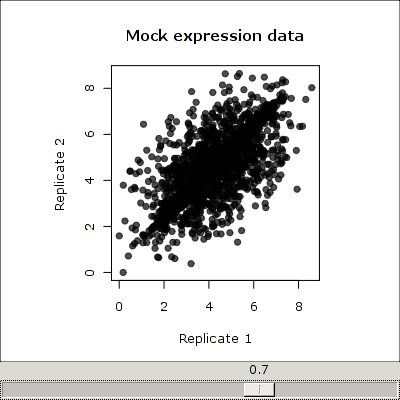
\includegraphics[width=3in]{demo-alpha-random-07-3}
\caption{\label{fig:rgtk2-demo-initial}Scatterplot of two microarray
replicates,
with a slider widget underneath that controls the alpha level of the
points. This screenshot shows the initial alpha of $0.7$.
This value does not lead to a clear display of the density at each
location.
}
\end{center}
\end{figure}

\begin{figure}[h!tbp]
\begin{center}
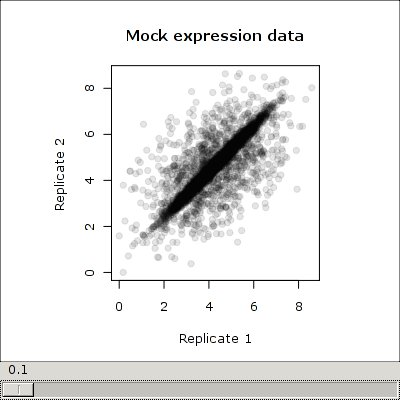
\includegraphics[width=3in]{demo-alpha-random-01-3}
\caption{\label{fig:rgtk2-demo-final}The same scatterplot from 
\ref{fig:rgtk2-demo-initial}, except the alpha parameter has been set
to to
$0.1$.}
\end{center}
\end{figure}

As a preliminary step, we use a 2D mixture distribution of correlated
variables to simulate expression values for two microarray chips. The
following code generates the data:
%DTL2:  Why are we not using real data?  And if we are using simulated
%data, why do we have to explain how in the code.  I would just say 
% here are the data
% MFL: so that readers may easily try this out for themselves
%DTL2:  make part of previous sentence or use a figure.
\begin{Code}
n <- 5000
backbone <- rnorm(n)
ma_data <- cbind(backbone + c(rnorm(3 * (n / 4), sd = 0.1), 
                              rt(n/4, 80)), 
                 backbone + c(rnorm(3 * (n / 4), , 0.1), 
                              rt(n / 4, 80)))
ma_data <- apply(ma_data, 2, function(col) col - min(col))
\end{Code}

The first step towards making our GUI is to create the window that
will contain the graphics device and slider widgets:
\begin{Code}
win <- gtkWindow(show = FALSE)
\end{Code}

One may embed \proglang{R} graphics within an \pkg{RGtk2} GUI using
the \pkg{cairoDevice} \citep{cairoDevice} package. The \pkg{cairoDevice} package draws
\proglang{R} graphics using \pkg{Cairo} \citep{cairo}, a library for
vector-based, antialiased graphics.  When \pkg{cairoDevice} draws to
the screen it is actually drawing to a \pkg{GTK+} widget of type
\code{GtkDrawingArea}. A \code{GtkDrawingArea} is an empty widget
meant for drawing arbitrary graphics in an interface. Here we
construct a drawing area in which the \proglang{R} graphics will be
drawn:
\begin{Code}
graphics <- gtkDrawingArea()
\end{Code}

Now that we have a widget for displaying \proglang{R} graphics, we
need the slider that controls the alpha level. A slider is a widget,
much like a scroll bar, for choosing a number at a certain precision
from a certain range. Here, a horizontal slider, called
\code{GtkHScale}, is created with a range from 0.1 to 1.0, with a
step size of 0.1:
\begin{Code}
slider <- gtkHScale(min = 0.1, max = 1.00, step = 0.1)
\end{Code}

When the user moves the slider, the plot should be updated so that its
alpha level reflects the slider value. This is achieved by connecting
an \proglang{R} callback function to the \code{value-changed} signal
of the slider, as in the code below:
%DTL2:  Goot to mention what type is the variable range here? a
%GtkRange as opposed to the use of the word range in the text meaning 
% a mathematical interval.
\begin{Code}
scale_cb <- function(range) {
              par(pty = "s")
              plot(ma_data[, 1], ma_data[, 2], 
                   col = rgb(0, 0, 0, alpha = range$getValue()),
                   xlab = "Replicate 1", ylab = "Replicate 2", 
                   main = "Mock expression data", pch = 19)
            }
gSignalConnect(slider, "value-changed", scale_cb)
\end{Code}
The callback function, \code{scale\_cb}, replots the
microarray data, \code{ma\_data}, using an alpha level equal to the
current value of the slider.
%DTL: It would be good to address the issues of global variables and
%the use of closures.
%ML: It seems you have well-formed thoughts on that issue; could you
%please add something?
%XXXX - for me.
%DTL2: I haven't had a chance to yet. Will do shortly.

The next steps are to add the drawing area and the slider to the
window and then to show the window on the screen. Although the window
is a container, it inherits from \code{GtkBin}, meaning that it can
hold only a single child widget. Thus, we will pack our widgets into a
vertical stacking box container, \code{GtkVBox}, and add our box to
the window.  Here, we would like the graphics to take up all of the
space not consumed by the slider, so the graphics device is packed to
\code{expand} and \code{fill}, while the slider is not
(See Section~\ref{sec:layout}). The following code performs the
packing operation:
%DTL2: connect to previous sentence of make separate figure.
\begin{Code}
vbox <- gtkVBox()
vbox$packStart(graphics, expand = TRUE, fill = TRUE, padding = 0)
vbox$packStart(slider, expand = FALSE, fill = FALSE, padding = 0)
win$add(vbox)
\end{Code}

As a final step, we set the default size of the window and show it and
all of its children:
\begin{Code}
win$setDefaultSize(400,400)
win$showAll() 
\end{Code}

Now that the window is visible on screen, we can instruct \proglang{R}
to draw its graphics to the drawing area using the
\code{asCairoDevice} function in the \pkg{cairoDevice} package:
\begin{Code}
require(cairoDevice)
asCairoDevice(graphics)
\end{Code}
%DTL2: The par(pty = "s") is specific to our application, and
%shouldn't it be done in the callback when doing the plotting just in
%case anybody (e.g., another callback) manages to put another plot
%there with different settings.
%moved
The call to \code{asCairoDevice} creates an \proglang{R} graphics
device from our drawing area widget and makes the device active, so
that it is the target of \proglang{R} plotting commands.

Finally, the value of the slider is initialized to $0.7$,
\begin{Code}
slider$setValue(0.7)
\end{Code}
which in turn activates the callback, generating the initial plot. The
initial state of the interface is shown in Figure~\ref{fig:rgtk2-demo-initial}.  Figure~\ref{fig:rgtk2-demo-final} shows
the plot after the user has moved the slider to set the value of alpha
to $0.1$.


\section{Sample application}\label{sec:spreadsheet-example}

The interfaces presented thus far are each designed for a singular,
focused task, such as choosing a CRAN mirror or viewing a scatterplot
at different alpha levels.  However, an interface often supports a
larger collection of separate operations, and the user is in control
of initiating different tasks from the general interface. These
interfaces for broader, more complex
applications are typically based on what is called an
%DTL: Here we define application window, yet we referred to it
%earlier.
\emph{application window}, which often contains a menu bar, tool bar,
application-specific area, and status bar in order from top to
bottom. The menu bar and tool bar are widgets designed to facilitate
the user selecting different \emph{actions}, each of which represents
an option or operation in the application.  The status bar at the
bottom commonly reports information about the activities or state of
the application or information for the user as a text message and may
be adjacent to a progress bar that displays the continuing progress of
long running operations.  This layout and design is a common
convention which helps users navigate a new GUI.


The following example demonstrates how one might construct a
reasonably complex
application using \pkg{RGtk2}. We aim to build a viewer for one or
more \proglang{R} \code{data.frame}s that is capable of sorting and
filtering the
rows in each \code{data.frame}. We also give it facilities to load and
save a \code{data.frame} to and from a CSV file. 

The resulting GUI is shown in Figure~\ref{fig:spreadsheet}. Each
\code{data.frame} frame is displayed in a table, using a
\code{GtkTreeView} widget. As we would like to support multiple
spreadsheets at once, we embed each table in a tabbed notebook,
\code{GtkNotebook}. Below each spreadsheet is a text entry (a
\code{GtkEntry} widget), in which the user may enter an expression for
filtering the table view. Below this is a status bar (a
\code{GtkStatusbar} widget) that communicates the status
of the application to the user, such as whether the loading of a
dataset is complete. At the top are a menu bar (a \code{GtkMenubar}
widget) and tool bar (a \code{GtkToolbar} widget) that allow the user
to invoke various actions, such as loading a new dataset or quitting
the application.

%DTL: the reader has to pull together the different parts in the next
%few pages.  It would be very valuable to provide a brief high-level
%overview of
%the steps involved and how they piece together and then go into the
%details.

% ML: I hope the paragraph above rectifies this.

%DTL2:  Yep, that helps. It would be useful I think also to
%identify/label the paragraphs that correspond to this different
%elements so that readers can quickly jump between them.
% Or as I have in my notes, 
%  Detail the steps in an intial short list at the beginning and then
%  label the intial paragraph/section for the topic with the
%  corresponding name.
%
% MFL: added a lot more structure to this section

% (BTW, statusbar, menu bar, etc. are not in the dictionary, so I
% changed (some of) them to status bar, menu bar, ....
% MFL: thanks, took care of the rest of them

% As it stands, this looks quite involved and will be intimidating.
% As for the XML, I think mentioning that is a big mistake.

% ML:
% I was intending for this example to be complex, in order to satisfy
% the readers that want to write a similar application in R. I thought
% the previous examples were sufficient to help users get started.
% Granted, there is a jump here, but I'm trying to satisfy a broad
% spectrum of readers.




\begin{figure}[h!tbp]
\begin{center}
%DTL:  The number of decimal places in this figure is way too
%much. Only wt has some values with 3 digits after the decimal.  So
% the remaining 3 are spurious, suggesting greater precision than the
% data support and for all the other variables, there are 4 or more
% unnecessary digits which serve only to obscure the meaningful ones.
%ML: This is a difficult problem to solve. Either we convert the data
% to a string ourselves (which would break eg sorting) or add an R
% handler to do the conversion on the fly (more complicated and slow).

%DTL2: Indeed, but it is something that people would expect to be able
%to control and something that immediately catches the eye as being
%not quite right. I assume a Cell Renderer would do the job as it is 
% a view of the model in the MVC framework. And if this does slow
% things down too much, that is a real limitation of Gtk+/RGtk and
% something we need to admit to, i.e., that this example is not
% suitable for
% large datasets and one should use, e.g., Gnumeric or a dedicated
% spreadsheet. But I think it is good to try it and if it is slow, we
% could figure out where and how to make it faster.
% But to ignore the problem suggests that the results one can achieve
% are less than professional quality. That is the case in so many R
% GUI papers and applications, so it would be nice to set a better
% tone and standard.
%
% MFL: I went ahead and added the callback to override the formatting.
% It is definitely slower, so I added a note about that.

%DTL2:  It would also be good to show multiple data sets in the screen
%shot. The fact that we talk about the ability to handle more than one
%and only show one is odd.  And it would also help to illustrate the
%notebook and its tabs.
% MFL: done

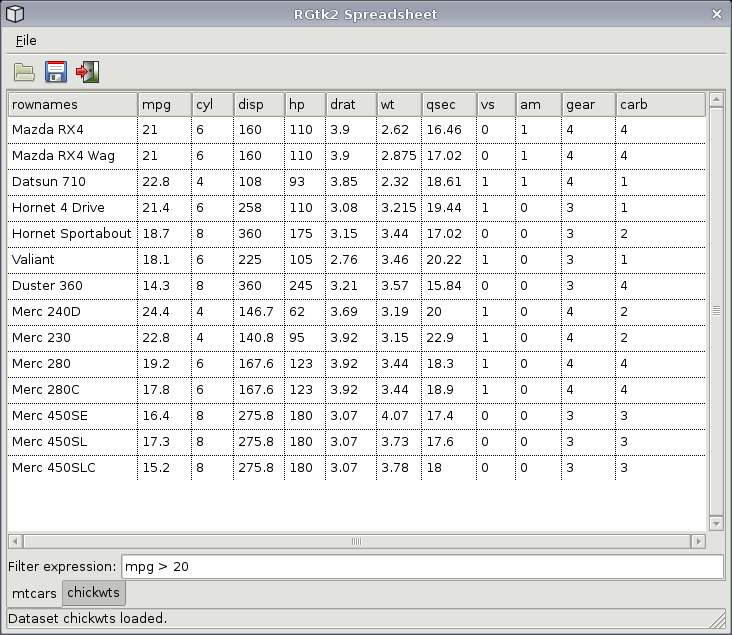
\includegraphics[width=6in]{spreadsheet.png}
\caption{\label{fig:spreadsheet}Screenshot of a spreadsheet
  application constructed with \pkg{RGtk2}. The current sheet is from
the
  \code{mtcars} dataset. The table is filtered by the expression
  \texttt{mpg > 20} and sorted by in decreasing order of the values of
the \code{mpg} variable.}
\end{center}
\end{figure}

\subsection{Main window}

We begin by creating the main window for the application and setting
its default size, specified in number of screen pixels:
%DTL2: Perhaps dynamically set the window title to the name of the
%dataset currently being viewed, i.e., when we switch tabs.
\begin{Code}
main_window <- gtkWindow(show = FALSE)
main_window["title"] <- "RGtk2 Spreadsheet"
main_window$setDefaultSize(600, 600)
\end{Code}

\subsection{Menu bar and tool bar}
\label{sec:spreadsheet-menubar}

Our spreadsheet application will support three user actions: open, save and quit. All three actions will be made available in both the menu bar and tool bar. Providing a user action requires (1)~implementing a callback function, (2)~defining the action properties, and (3)~manifesting the action as a widget in the GUI. We consider each of these steps in turn.

\subsubsection{Implementing the callbacks}

We begin by implementing the callbacks corresponding to the user
actions. operations for the menu items and corresponding
callbacks to load and save a \code{data.frame} and to quit the
``application'':
\begin{Code}
open_cb <- function(widget, window)  
{
  dialog <- gtkFileChooserDialog("Choose a CSV file", window, "open",
                                 "gtk-cancel",
                                 GtkResponseType["cancel"],
                                 "gtk-open",
                                 GtkResponseType["accept"])
  if (dialog$run() == GtkResponseType["accept"]) {
    df <- read.csv(dialog$getFilename())
    load_spreadsheet(df, basename(dialog$getFilename()))
  }
  dialog$destroy()
}
save_cb <- function(widget, window) {
  dialog <- gtkFileChooserDialog("Enter a name for the file", window,
                                 "save",
                                 "gtk-cancel",
                                 GtkResponseType["cancel"],
                                 "gtk-save",
                                 GtkResponseType["accept"])
  if (dialog$run() == GtkResponseType["accept"])
    save_file(dialog$getFilename())
  dialog$destroy()
}
quit_cb <- function(widget, window) 
              window$destroy()

\end{Code}
Each of these functions is a callback which takes the widget
associated with the action as its first argument and the
top-level window as its second. The load and save operations leverage
the \code{GtkFileChooserDialog} widget type, a dialog that contains a
graphical file browser for specifying the path to a
file. \code{GtkFileChooserDialog} has several modes corresponding to
common file selection tasks. In this case, we use the \code{open} mode
for the reading action and the \code{save} mode for the writing
action. The \code{accept} response from the dialog indicates that the
user has confirmed the file selection by clicking the \code{Open} or
\code{Save} button.

\subsubsection{Defining the actions}

We now define the actions that will delegate to the callbacks
implemented above. The \code{GtkAction} class represents an operation
that a user may request an application to perform. A \code{GtkAction}
instance may be manifested as a widget in multiple ways, such as an
item in a menu or a button in a tool bar. The widgets are synchronized
with the properties of the \code{GtkAction}. For example, if an action
is disabled, the menu items and tool bar buttons will also be
disabled. Extensions of \code{GtkAction} exist for toggle and radio
options, but those are not described here. For details, see
\code{help(GtkToggleAction)} and \code{help(GtkRadioAction)},
respectively. A \code{GtkActionGroup} is a container for
\code{GtkAction} objects. 
% DTL: I think the concept of a GtkAction needs more description here,
% just the basic idea.

In the following code, we define the actions for our application and
bundle them into a \code{GtkActionGroup}:
\begin{Code}
actions <- list(
  list("FileMenu", NULL, "_File"), 
  list("Open", "gtk-open", "_Open File", "<control>O", 
       "Select a CSV file to load as a spreadsheet", open_cb),
  list("Save", "gtk-save", "_Save", "<control>S", 
       "Save the current spreadsheet to a CSV file", save_cb),
  list("Quit", "gtk-quit", "_Quit", "<control>Q", 
         "Quit the application", quit_cb)
)
action_group <- gtkActionGroup("spreadsheetActions")
action_group$addActions(actions, main_window)
\end{Code}
Above, each action is defined with a list, containing the action ID
(for referring to the action later in the code),
% Is this for referring to it later or the label that appears in the
% tool bar and/or menu bar?
% DTL2: What does "stock" mean here? I think it is tied to the Gtk+
% documentation, but doesn't tell us much. So perhaps just omit and
% use icon separately.
icon ID, label, keyboard shortcut, tooltip, and callback. The first
action will serve as the basic menu container
% DTL: this is vague and undefined so please explain.
for the rest of the items and actions. Since it performs no
function, it is not necessary to specify all of the fields,
such as the callback. 

%DTL2: Can you add a reference
%DTL2: Put this in a figure or connect to a sentence.
%DTL2:  It would be good to use formal classes or at least named
%elements here rather so that the reader of the code knows what each 
% element is for. For example, one cannot figure out what the NULL is
% for.
% MFL: I moved the description of the elements to before the example.
% I hope this makes it clearer.

%DTL:  If the FileMenu element is a container for the Open, Save and
% Quit elements, why aren't they elements of the FileMenu list.
% This flat structure to represent a hierarchy seems odd.
%ML: In GTK+, the actions are not organized hierarchically - that is
% specified in the layout (which is parsed from XML).
Specifying the action definitions as \proglang{R} lists is an example
of  high-level type conversion, where a native \proglang{R} structure
is implicitly converted to a complex \pkg{GTK+} object. In this case,
an \proglang{R} list is being converted to a set of \code{GtkAction}
objects. See Section~\ref{sec:type-conversion} for
a technical explanation and justification.

\subsubsection{Creating widgets for the actions}

In order to make these actions available to the user, they need to be
mapped to a widget in the GUI. \pkg{GTK+} provides a class known as
\code{GtkUIManager} to facilitate this operation. In the following
code, we create a \code{GtkUIManager} instance and register our
actions with it:
\begin{Code}
ui_manager <- gtkUIManager()
ui_manager$insertActionGroup(action_group, 0)
\end{Code}
Next, we specify
the layout of the menu bar and tool bar containing the actions defined
above, by calling the \code{gtkUIManagerAddUi} method: 
%DTL:  Boy, this seems very odd. Why an R programmer would switch to
%XML to express something that is easily specified in R is bizarre.
% I think you will really turn people off with this. Some people have 
% a strong  (often unfounded) objection to XML and this will allow
% them to discard RGtk2.  The XML is a red-herring. And it makes for
% a very big discontinuity in the programming style for creating a
% GUI, changing syntax, etc.
%ML: I've changed this to use the low-level API
% It's not as pretty but will keep everything in R.
% Could try to express a subset of it as a list... not sure.
%DTL2: Thanks. I think it is better.  
\begin{Code}
merge <- ui_manager$newMergeId()
ui_manager$addUi(merge.id = merge, path = "/", name = "menubar",
                 action = NULL, type = "menubar", top = FALSE)
ui_manager$addUi(merge, "/menubar", "file", "FileMenu", "menu", FALSE)
ui_manager$addUi(merge, "/menubar/file", "open", "Open", "menuitem", FALSE)
ui_manager$addUi(merge, "/menubar/file", "save", "Save", "menuitem", FALSE)
ui_manager$addUi(merge, "/menubar/file", "sep", NULL, "menuitem", FALSE)
ui_manager$addUi(merge, "/menubar/file", "quit", "Quit", "menuitem", FALSE)
ui_manager$addUi(merge, "/", "toolbar", NULL, "toolbar", FALSE)
ui_manager$addUi(merge, "/toolbar", "open", "Open", "toolitem", FALSE)
ui_manager$addUi(merge, "/toolbar", "save", "Save", "toolitem", FALSE)
ui_manager$addUi(merge, "/toolbar", "quit", "Quit", "toolitem", FALSE)
\end{Code}
Each piece of the user interface added to a \code{GtkUIManager}
instance must be associated with a
\emph{merge id}, as retrieved from \code{gtkUIManagerNewMergeId}. It
is passed to \code{gtkUIManagerAddUi} as the \code{merge\_id}
parameter. This allows removing (unmerging) the UI in batch at a later
time. The \code{path} parameter indicates where the UI element should
be merged. Similar to a path in a file system or URL, each element
name in the path is delimited by a forward slash (``/''). The
\code{name} parameter identifies the element to the manager, and
\code{action} is the ID of the action in the provided action group.
The ID can be \code{NULL} in the case of containers (menu bars and
tool bars) and separators. Finally, \code{type} indicates the type of
UI element, such as a tool bar or menu bar. The default is
\code{auto}, which asks the \code{GtkUIManager} to guess based on the
path.
%DTL2:  I don't think declarative is the right term here.
% In what way is XML more declarative than R or any programming
% language.
% I think the key idea where XML is preferred is that it is generated
% by another tool or already exists in a language neutral manner 
% and so can be readily reused in an arbitrary language. But for
% building a GUI ourselves in R, an XML "document" is not convenient.
%MFL: Well the XML is definitely clearer to me than the 
% mess above. BUT I agree with you in general. There needs to be
% a better solution.
% I took out the XML comment.

The next step is to use the \code{GtkUIManager} to create the actual
menu bar and tool bar widgets from the action definitions and layout.
\begin{Code}
menubar <- ui_manager$getWidget("/menubar")
toolbar <- ui_manager$getWidget("/toolbar")
main_window$addAccelGroup(ui_manager$getAccelGroup()) 
\end{Code}
The final line above enables keyboard shortcuts in the main window.

\subsection{Status bar}

To report information from and about the application, we will use a
\code{GtkStatusbar} widget.  A status bar maintains a 
% DTL2: You probably need to explain (in one sentence) what a stack is
% in this context.
stack of text messages and displays the message on top of the
stack. When a message is added to the status bar stack, it is
immediately displayed, and when the message is removed, the previous
one is displayed.
%DTL2: e.g., When we add a message, it is immediately displayed and
%when we remove it, the previous one is then displayed.
Each message is associated with a \emph{context}, and each context has
its own ID. A context ID is a number that is generated in a consistent
way from any user-supplied string that serves as the human-readable
context name.  A context ID may be created using the
\code{gtkStatusbarGetContextId} function.
Here we create a status bar and push the message \code{"Ready"} onto
the top of the stack within the context named \code{"info"} (other
contexts could be named, e.g.,
\code{"warning"} or \code{"error"}):
%DTL2: It is not quite obvious what the R variable info is - a context
%or an ID.  We are getting the ContextId but it seems like the "info"
%is the Id and we get the Context.
\begin{Code}
statusbar <- gtkStatusbar()
info <- statusbar$getContextId("info")
statusbar$push(info, "Ready") 
\end{Code}

\subsection{Spreadsheet panel}
\label{sec:spreadsheet-panel}

Next, we need to create the \code{GtkTreeView} that will display a
given \code{data.frame} as a table.  The data is first loaded into a
\code{GtkTreeModel}, from which the \code{GtkTreeView} retrieves the
values it displays. Below each sheet is a text entry box for entering
an expression for filtering the spreadsheet rows. All of the open
sheets will be placed within notebook-style container.

\subsubsection{Data model}

The following function, \code{create\_tree\_model}, will create a
\code{GtkTreeModel} object that obtains its data from an \proglang{R}
\code{data.frame}, passed as an argument to the function:
%DTL2: Connect the code to the previous sentence, i.e., : or figure
% and put a comment or two in the code to make it clearer/more
% accessible to the reader.
\begin{Code}
create_tree_model <- function(df) {
  df <- cbind(rownames = rownames(df), df)
  filter_df <- cbind(filter = TRUE, df)
  model <- rGtkDataFrame(filter_df)
  filter_model <- gtkTreeModelFilterNew(model)
  filter_model$setVisibleColumn(0)
  sort_model <- gtkTreeModelSort(filter_model)
  sort_model
}
\end{Code}
The function employs the \code{RGtkDataFrame} utility that allows
the \code{GtkTreeView} to use an \proglang{R}
\code{data.frame} as its data source.
%DTL2: model is a dangerous term to use in statistics as many will
%think it refers to a statistical model!
% You could use the word "source".  If you stick with model, then you
% need to have a reference and a brief sentence about the Model View
% Controller paradigm.  Many readers will not be familiar with that
term.
In order to support filtering
and sorting of the displayed data, the \code{RGtkDataFrame} is proxied
by a \code{GtkTreeModelFilter} model, which in turn is proxied by a
\code{GtkTreeModelSort} model. A proxy data model sits between a
source data model and a client, such as a \code{GtkTreeView}. The data
provided by a proxy model results from the modification of the data in
the source model.
%DTL2: Does the proxy actually modify the source or just represent a
%modified view of the original source? This is an issue for R as it
%has no references and does not have side-effects (in general).
% MFL: No it does not modify the source.

\subsubsection{Table view}

The next function, \code{create\_tree\_view},  will create the
\code{GtkTreeView} given the \code{GtkTreeModel} created by
\code{create\_tree\_model} above:
\begin{Code}
create_tree_view <- function(model) {
  tree_view <- gtkTreeView(model)
  rdf <- model$getModel()$getModel()
  sapply(tail(seq_len(ncol(rdf)), -1), function(j) {
    renderer <- gtkCellRendererText()
    column <- gtkTreeViewColumn(colnames(rdf)[j], renderer, 
                                text = j - 1)
    column$setSortColumnId(j - 1)
    column$setCellDataFunc(renderer, 
                           function(column, renderer, model, iter) 
    {
      iter <- model$convertIterToChildIter(iter)$child.iter
      child <- model$getModel()
      iter <- child$convertIterToChildIter(iter)$child.iter
      i <- rdf$getPath(iter)$getIndices()[[1]] + 1
      renderer["text"] <- as.character(rdf[i, j])
    })
    tree_view$appendColumn(column)
  })
  tree_view$setHeadersClickable(TRUE)
  if (is.null(gtkCheckVersion(2, 10, 0))) 
    tree_view$setGridLines("both")
  tree_view
}
\end{Code}
Above, each column of the \code{data.frame},
provided as the second argument, is displayed by a column in the tree
view. We configure the tree view so that it shows grid lines (if the
user has \pkg{GTK+} 2.10.0 or higher) and supports sorting on a column
when the user clicks on the column header.
The call to \code{setCellDataFunc} attaches a callback that formats
the text values as \proglang{R} does by default (\pkg{GTK+} takes a
simpler approach that gives each number 6 significant figures). Note
that this callback is called each time a cell is rendered, so it could
negatively impact performance, especially when scrolling. For large
spreadsheets, we recommend using a dedicated spreadsheet application. 

%DTL:  why doesn't gtkCheckVersion() return TRUE or FALSE? Checking
% for NULL is a little counter-intuitive.
%ML: I agree, but I don't want to get into the business of redesigning
% the GTK+ API.
%DTL2: Fair enough.

\subsubsection{Filter text entry}

Next, we define a function that creates the text box for the user to
enter a filter expression:
%DTL: It is not clear to me why you are assigning a function and then
% referring to it when it is never used again. Why not put the
% function definition in the call to gSignalConnect()?
\begin{Code}
create_entry <- function(model)
{
  entry <- gtkEntry()
  gSignalConnect(entry, "activate", 
                 function(entry) {
                   model[, "filter"] <<- 
                    eval(parse(text = entry$text), 
                         as.data.frame(model))
                 })
  entry
}
\end{Code}
This uses the \code{GtkEntry} widget.
Whenever the \code{GtkEntry} is ``activated,'' e.g., by the user
pressing the \texttt{ENTER} key, we update the filter by the result of
the \proglang{R} expression.
%DTL2:  Does this do the right thing or do you need <<- rather than
% <-. This is a closure and you are
%modifyng the value of model. But a <- rather than <<- will make a
%local modification within the function call, not within the
%environment containing model. Is this a regular R object or an RGtk
%object pointing to a C object. Either way, <<- is probably best.
%MFL: It's an externalptr (an RGtkDataFrame), <<- is fine.

\subsubsection{Notebook of sheets}

In order to handle multiple spreadsheets simultaneously but display
only one at a time, we will use a special type of container called
\code{GtkNotebook}.  This provides tabs on the border of the
notebook like a ring binder which the user can select to switch
between the different widgets within the notebook.  This is used in
Excel to present several work sheets within a single window, and also
within certain Web browsers to allow the user to view multiple Web
pages without opening multiple windows.

Below, we create the notebook:
\begin{Code}
notebook <- gtkNotebook()
notebook$setTabPos("bottom")
\end{Code}

\subsection{Integrating the components}

The menu bar, tool bar, spreadsheet notebook and status bar all need
to be contained within the main window. In the code below, we add each
of these components to the GUI by placing them inside a
\code{GtkVBox}:
\begin{Code}
vbox <- gtkVBox(homogeneous = FALSE, spacing = 0)
vbox$packStart(menubar, expand = FALSE, fill = FALSE, padding = 0)
vbox$packStart(toolbar, FALSE, FALSE, 0)
vbox$packStart(notebook, TRUE, TRUE, 0)
vbox$packStart(statusbar, FALSE, FALSE, 0)
main_window$add(vbox)
main_window$show()
\end{Code}

\subsection{Loading a spreadsheet}

Finally, we define the \code{load\_spreadsheet} function, as called
from the \code{open\_cb} callback above, that loads a
\code{data.frame} into the GUI:
%DTL2:  make the connection between this code and the callback for
%open_cb which is 3 1/2 pages back. 
%DTL2: connect to sentence or put in figure.
\begin{Code}
load_spreadsheet <- function(df, name) {
  model <- create_tree_model(df)
  tree_view <- create_tree_view(model)
  entry <- create_entry(model$getModel()$getModel())
  
  hbox <- gtkHBox(FALSE, 5)
  hbox$packStart(gtkLabel("Filter expression:"), FALSE, FALSE, 0)
  hbox$packStart(entry, TRUE, TRUE, 0)
  vbox <- gtkVBox(FALSE, 5)
  scrolled_window <- gtkScrolledWindow()
  scrolled_window$add(tree_view)
  vbox$packStart(scrolled_window, TRUE, TRUE, 0)
  vbox$packStart(hbox, FALSE, FALSE, 0)

  if (missing(name))
  name <- deparse(substitute(df))
  notebook$appendPage(vbox, gtkLabel(name))
  
  statusbar$push(info, paste("Dataset", name, "loaded."))
}
\end{Code}
This function creates the necessary
widgets and packs them into a notebook page. To limit its visible
size, the data grid/table is added to a \code{GtkScrolledWindow}.
The function concludes by updating the status bar to indicate that the
dataset has been successfully loaded. 

An example of using the above function to add a spreadsheet is given
below:
\begin{Code}
load_spreadsheet(mtcars)
\end{Code}

This application is obviously missing many important features. For
example, there is no easy way to return to the complete
\code{data.frame} after subsetting, and
it is not possible to edit the cells. The main purpose of the example
is to introduce the process of building an application window.

\section{Advanced features}

This section describes features of \pkg{RGtk2} that are beyond the
construction of basic and intermediate GUIs. It is meant for readers
interested in advanced and specialized \pkg{RGtk2} features such as
the ability to extend \pkg{GTK+} classes and interface with low-level
and third-party libraries that are integrated with \pkg{GTK+}. Much of
this functionality is applicable outside of GUI construction.

%DTL: say who the intended audience is so that readers know if it is
%for them. The material on types & classes is advanced but not in the
%sense of more complex GUIs, but for a whole different type of RGtk
%user.

First, we describe the additional libraries (other than \pkg{GTK+})
bound by
\pkg{RGtk2} that are meant to support the construction of advanced,
graphically-intensive interfaces. The focus then shifts to the
low-level support for the \pkg{GObject} object-oriented programming
library. The \pkg{RGtk2} user is able to manipulate objects in
external \pkg{GObject}-based applications (i.e., top-level GUIs running
within the same \proglang{R} session) that are bound to \proglang{R}
by code
outside of the \pkg{RGtk2} package. \pkg{RGtk2} also supports defining
new \pkg{GObject} classes in \proglang{R}.

\subsection{Additional library support}

The \pkg{GTK+} 2.0 library incorporates several other libraries:
\pkg{Cairo}, \pkg{GDK}, \pkg{GdkPixbuf}, \pkg{Pango} and \pkg{ATK}. 
%each of which we describe below. 
The \pkg{RGtk2} package provides \proglang{R}-level bindings for
these libraries, in addition to \pkg{GTK+} itself. The following
sections describe the purpose and functionality of each library.

\subsubsection[Cairo]{\pkg{Cairo}} 

Cairo is a 2D vector graphics library with which \pkg{GTK+} widgets
%DTL2:  Is it really for drawing the widgets themselves or used for 
% drawing onto Gtk widgets?
%MFL: The widgets themselves - GTK+ uses Cairo for all drawing
are drawn. It is possible to use \pkg{Cairo} directly to draw custom
graphics within a \code{GtkDrawingArea}. The library is also useful
outside of GUI construction, in that one can draw vector graphics to
off-screen surfaces in common formats such as PNG, SVG, PS, and PDF
files.

\subsubsection[GDK]{\pkg{GDK}}

The GIMP Drawing Kit, \pkg{GDK}, is the low-level hardware access and
drawing layer 
%DTL2:  Since Cairo is also for drawing, need to mention why Gdk has
%drawing facilities also.
for \pkg{GTK+}. It is most useful for raster-based (non-vector)
drawing of graphical primitives like lines, rectangles and circles and
for handling raw mouse and keyboard events. It also provides access to
windowing system resources, such as screens in a multi-headed
environment. Although the drawing functions of \pkg{GDK} overlap
somewhat with \pkg{Cairo}, \pkg{Cairo} is for drawing vectors, while
\pkg{GDK} is for direct drawing of pixels. Another reason for the
redundancy is that \pkg{GDK} predates \pkg{Cairo}, and thus the
\pkg{GDK} drawing routines are present for backwards compatibility.

\subsubsection[GdkPixbuf]{\pkg{GdkPixbuf}}

\pkg{GdkPixbuf} is an image manipulation library based on \pkg{GDK}.
Its features
include rendering, scaling, and compositing of images. \pkg{GdkPixbuf}
can read
and write several image formats, including JPEG, PNG, and GIF. Like
\pkg{Cairo},
\pkg{GdkPixbuf} could be used independently of a GUI for working with
arbitrary 
graphics in \proglang{R}. 
%DTL: This doesn't seem very relevant at this point.
%The \pkg{RGdkPixbuf} \citep{RGdkPixbuf} package bound
%the previous generation of \pkg{GdkPixbuf}.

\subsubsection[Pango]{\pkg{Pango}}

\pkg{Pango} provides facilities for rendering and formatting text with
rich capabilities for handling international characters. It also
provides cross-platform access to the font configuration of a system.
\pkg{Pango} is most often used directly for embedding text in graphics
when drawing to a \code{GtkDrawingArea} or an off-screen destination,
e.g., image.

\subsubsection[ATK]{\pkg{ATK}} 

The Accessibility ToolKit (\pkg{ATK}) supports accessibility
technologies to make GUIs amenable to users with ``disabilities''.  It
allows accessibility devices to interact with \pkg{GTK+}
GUIs. \pkg{ATK} is not likely to be very useful from \proglang{R}. Its
binding is included for the sake of completion, since \pkg{ATK} types
are present in the \pkg{GTK+} API.

\subsubsection[Libglade]{\pkg{Libglade}}

\pkg{Libglade} constructs \pkg{GTK+} GUIs from \proglang{XML}
descriptions.
The \proglang{XML} descriptions are output from
\pkg{Glade}, which is a GUI tool for interactively designing other
GUIs. 
%The \pkg{RGtkGlade}
%package \citep{RGtkGlade} bound the previous generation of this
%library.
As of \pkg{GTK+} 2.12.0, which includes native support for
constructing widgets from \proglang{XML} descriptions, \pkg{Libglade}
is
essentially obsolete. The bindings are still included for backwards
compatibility.

\subsection[GObject primer]{\pkg{GObject}
primer}\label{sec:primer}

\pkg{GTK+}, as well as the libraries described in the previous
section, except for \pkg{Cairo}, are based on the \pkg{GObject}
library for object-oriented programming in \proglang{C}. \pkg{GObject}
forms the basis of many other open-source projects, including the
\pkg{GNOME} \citep{GNOME} and \pkg{XFCE} 
\citep{xfce} desktops and the \pkg{GStreamer} multimedia framework
\citep{gstreamer}.

\pkg{RGtk2} interfaces with parts of \pkg{GObject} and permits the
\proglang{R}  programmer to create new \pkg{GObject} classes in
\proglang{R}. Understanding this functionality depends on a
familiarity with the concepts underlying 
\pkg{GObject}. This section introduces those concepts.

\pkg{GObject} is organized as a collection of modules. The fundamental
modules are \code{GType}, \code{GSignal}, and the base
\code{GObject} class. Each of these modules is described in the
following sections. For further details, please see the \pkg{GObject}
documentation \citep{gobject}.

\subsubsection{\code{GType}}
% DTL: This is very detailed but more in a factual way than an
% informative way, especially the GObject material. When reading it, I
% wasn't certain what was going on and I know this stuff. In fact,
% this is the standard way of doing OOP in C (with the type formalism
% added), i.e., struct nesting to get field offsets to align for
% inheritance and function pointers. Similarly, the concept of an
% interface being similar to that of many other languages gets lost
% and the details obscure the concept.  The essential idea is that it
% it is a constraint and a contract to ensure that a "type" provides
% particular methods but does not provide them via inheritance or any
% constraint on the physical representation of that class.
%
% ML: Good points.  I tried to address these issues.

% It would also be better if you explain earlier why the reader needs
% to know this stuff, i.e., where are you going with it in the paper.

% ML: This is mentioned in the section above. Does it need more?

\code{GType} is at the core of \pkg{GObject}. Its basic purpose
is to manage the definition, registration and introspection of types
at run-time. The main commonality between all \code{GType}s is that
they define a method for copying their values. This allows generic
memory management for every value with a \code{GType}. Those
\code{GType}s that directly define a copy mechanism, instead of
inheriting one, are known as \emph{fundamental} \code{GType}s.

% MFL2: I tried to simplify this some more and improve its clarity.

The set of fundamental \code{GType}s includes many of the built-in
\proglang{C} data types. For example, ``primitive'' types like
integers, doubles, and strings (character pointers) are all
fundamental \code{GType}s. 

Arbitrary \proglang{C} structures are adapted to the \code{GType}
framework by providing a copy function and free function for the
structure. Such \code{GType}s are said to be \emph{boxed} and inherit
from the fundamental \code{GType} called \code{GBoxed}. For
example, \pkg{RGtk2} registers a boxed \code{GType} for the
\proglang{R} \code{SEXP} structure, which is used to represent all
\proglang{R} objects in \proglang{C}.

The \code{GType} module also supports the definition of object types
(the main purpose of \pkg{GObject}). Like all \code{GType}s, object
\code{GType}s must be or inherit from a fundamental \code{GType}.
\pkg{GObject} provides a fundamental \code{GType}, \code{GObject},
that may be extended to define a new type of object. Every
\code{GType} derived from \code{GObject} has a \proglang{C} structure
representing its class. Inheritance of class structures is
accomplished through the standard \proglang{C} idiom for
object-oriented programming: prefixing a structure with the structure
of the parent class, so that fields are aligned. The use of the
structure prefixing idiom restricts \pkg{GObject} to single
inheritance. The class structure contains class-wide fields, including
function pointers called \emph{virtual functions} that may be
overriden by changing the value of the corresponding field in the
class structure during intialization. This is the primary mechanism in
\pkg{GObject} for changing class
%DTL2: Is this object or class. Presumably class and hence the
%behaviour of all objects of that class. 
behavior through inheritance. Each object \code{GType} also has a
registered structure with instance-level members (i.e., fields). The
instance structure of a \code{GType} inherits from the parent instance
structure using the same idiom as the class structures. An instance of
an object \code{GType} is manifested as a value of the corresponding
instance structure. In order to link an instance to its class, each
instance structure holds a reference to the shared value of the class
structure for the \code{GType}.

Like many object-oriented languages, \pkg{GObject} supports the
definition and implementation of \emph{interfaces}. An interface
specifies a set of methods that represent a role performed by one or
more classes, where the role is shared independently of the class
hierarchy. If a class plays a role represented by an interface, it may
formally declare the contract by registering itself as an
implementation of the interface. As a result, the type is required to
provide values (implementations) for the methods declared by the
interface. Any object \code{GType}, such as \code{GObject},
may implement multiple interfaces. Like a \code{GObject}-derived
\code{GType}, an interface has a class structure that declares its
virtual functions (i.e., methods). Every interface class structure may
only be prefixed by \code{GTypeInterface}, so there is no inheritance
between interfaces in \pkg{GObject}. This is a significant difference
from many object-oriented languages. However, an interface can be made
to \emph{require} the implementation of one or more other interfaces
by any \code{GType} that implements it. Unlike \code{GObject},
\code{GTypeInterface} is non-instanciable, so there is no
instance-level structure and it is not possible to create instances of
interfaces directly.

Two other fundamental \code{GType}s are
\code{GEnum} and \code{GFlags}, both of which are registered with a
class structure. The \code{GEnumClass} structure stores metadata about
a particular enumeration, such as the names and nicknames of its
values. \code{GFlags} is similar as it represents an enumeration
where the values are intended to be combined bitwise (via \code{AND} and \code{OR}
operations) to represent the presence of one or more settings.
%DTL2: technically not all have to be powers of two.

\subsubsection{\code{GSignal}}

One of the defining characteristics of \pkg{GObject} is its emphasis
on \emph{signals}, which were introduced earlier in this paper in the
context of notification of user events in a \pkg{GTK+} GUI. Any
instance of a \code{GType} can have registered signals. Each
\emph{signal} is defined by its name and the types of its arguments
and return value. A class inherits signals from its parents.

\subsubsection[GObject base class]{\code{GObject} base class}

\code{GObject} is the basic/fundamental classed and instanciable
\code{GType} provided by the \pkg{GObject} library.  The key feature
provided by the \code{GObject} class, from the perspective of the
\pkg{RGtk2} user, are \emph{properties}. Properties may be thought of
as introspectable and encapsulated public fields. Like instance fields
of a \code{GObject}-derived \code{GType},
%DTL2: in what context ? Gtk+, C, ...
properties
are inherited. They support automated validation of their values at
runtime, and a change in a property value emits the \code{notify}
signal from its instance, allowing objects to respond to changes in
the state of other objects. It is possible to control whether a
property is readable, writeable, and more. Depending on the options
specified in the declaration of a property,
%DTL2: declaration or optinons specified when it is declared
one may be able to or even restricted to set a property at
construction time, using the generic \code{GObject} constructor,
\code{gObject()}.

A property is defined by a \code{GParamSpec} structure that specifies
a name, nickname, description, value \code{GType}, and other options.
There are subclasses of \code{GParamSpec} for particular \code{GType}s
that permit specification of further constraints. For example,
\code{GParamSpecInt} is specific to integers and can be
configured to restrict its valid range of integer values between a
minimum and maximum. Many \code{GParamSpec} subclasses also permit
default values.

\subsection[Interfacing with external GObject-based
applications]{Interfacing with external \pkg{GObject}-based
applications}

Many of the \pkg{RGtk2} functions developed for the creation of GUIs
using \pkg{GTK+} are applicable to other libraries and applications
based on \pkg{GObject}. There are several such packages of interest to
staticians, including \pkg{Gnumeric}, a spreadsheet application, and
\pkg{GGobi}, software for multivariate interactive graphics. The
\pkg{rggobi} package \citep{rggobi} provides a high-level interface to
\pkg{GGobi} from \proglang{R}. Although it is somewhat hidden,
\pkg{rggobi} objects are \code{externalptr}s that reference the
underlying \pkg{GGobi} objects, which extend
\code{GObject}. \pkg{RGtk2} uses the same \proglang{R} representation,
so many \pkg{RGtk2} functions can operate on \pkg{rggobi} objects
directly without additional interface code.

As an example, we consider the problem of displaying an \proglang{R}
plot in response to a user ``identifying'' a point in a \pkg{GGobi}
plot with the mouse. When a \pkg{GGobi} point is identified, the main
\pkg{GGobi} context emits the \code{identify-point} signal. If we
connect an \proglang{R} function to this signal, using
\code{gSignalConnect}, the function will be executed whenever a point
is identified. 
%DTL: This code does not form part of a grammatical construct so is
%just "out" there. It should be in a figure if it is not in a
%sentence.
% Also, think it is better to introduce it first with a sentence or
% two describig the basic idea.
The following code displays data within a \pkg{GGobi} window and
draws a fit of the simple linear model in a separate \proglang{R}
graphics window in response to the user identifying a point:
%DTL2: Make a figure or connect to sentence.
\begin{Code}
library("rggobi")
attach(mtcars)
gg <- ggobi(mtcars)
model <- lm(mpg ~ hp)
plot(hp, mpg)
abline(model)
gSignalConnect(gg, "identify-point", 
               function(gg, plot, id, dataset) {
                plot(hp, mpg)
                points(hp[id + 1], mpg[id + 1], pch = 19)
                abline(model)
               })
\end{Code}
The \pkg{GGobi} instance is initialized with the \code{mtcars}
dataset.  A linear model is fit with \code{lm} and the line is drawn
on an \proglang{R} plot. The important step is connecting a handler to
the \code{identify-point} signal. The handler regenerates the
\proglang{R} plot, and, for the identified point, replaces the empty
circle glyph with a filled circle.  In this way, we have created a
simple integration of the interactive
graphics of \pkg{GGobi} with an \proglang{R} graphic that displays a
linear model fit, which \pkg{GGobi} cannot display. Since the
\pkg{GGobi} GUI is based on \pkg{GTK+}, it would also be possible to
embed the \pkg{GGobi} plot into an \pkg{RGtk2} GUI. More interesting
integration uses the same basic tools. Please see the \pkg{rggobi}
documentation for more details.

\subsection[Defining GObject classes]{Defining \pkg{GObject} classes}
\label{sec:classes}

All of the above examples utilize objects that are implemented in
\proglang{C}.
\pkg{RGtk2} supports the definition of \code{GObject}-derived classes
from within
\proglang{R}.  The \code{gClass} function in \proglang{R} registers a 
class, given the name of the new class, the name of the parent class,
and the class 
definition. The class definition is a series of arguments that specify
the new fields, new methods, 
%DTL: method overrides seems to be a idiosyncratic and customized
%word. It certainly needs a definition and again, the concept would be 
% better than assuming the reader can infer the meaning.
% I suggets using something like 
methods that override inherited methods,
%method overrides,
 signals, properties, and
initialization function
%DTL2:  function or functions. I think the latter, but please check.
%MFL2: 'functions' - there's one hook called during initialization
for the class. The name of a parameter specifies its role in the
definition.

\subsubsection{Example of defining a class}

The example below illustrates the definition of a new
\code{GObject}-derived
class by revisiting the example in Section~\ref{sec:embedded-graphics}
involving the embedded plotting of 
microarray data.
%DTL: Put a cross-reference/link back to that example. Is it really
%the first? I thought the CRAN example would be considered first.
The slider in that example controls the alpha level of the
points in the scatterplot in a linear fashion. Given the large amount
of
overplotting, the alpha level does not have a strong visual effect
until it
approaches its lower limit. One may desire greater control in this
region,
without limiting the range of the slider. 

A possible solution would be to map the slider value to an alpha value
using a non-linear function. All that is required is to change the
slider callback so that it computes the alpha value as a non-linear
function of the slider value. However, the label on the slider would
be inaccurate; it would still report the original value.  Overriding
how the label is computed is possible by connecting a handler
%DTL: connecting "what"?
to the
\code{format-value} signal on the \code{GtkScale} class. Let us
assume,
however, that we would like to create a reusable type of slider that
mapped its value using a specified \proglang{R} expression.

Below is our invocation of \code{gClass} that
defines \code{RTransformedHScale}, an extension of \code{GtkHScale},
the horizontal slider:
%DTL: First, the arguments to gParamSpec are not clear just by reading
%them. Why not use the parameter names, as in
%    gParamSpec(type = "R", name = "expr", nick = "e", blurb =
%"Transformation of scale value",
% That would make it clearer.
% Also, the  description in the paragraph that explains this code
% does not refer to the value "R" at all but to 
% RGtkSexp which presumably is synonamous with "R" but it is not
% clear.
% 
% Why do you need a list () for the third argument rather than have
% .props, .public, ... as named parameters. It is very un-R-like.
%
% ML: I was thinking that one might want to encapsulate the definition
% of a class within a list, but I agree that it is probably cleaner to
% make the function variadic. Thanks for the suggestion.
\begin{Code}
tform_scale_type <- gClass("RTransformedHScale", "GtkHScale",
  .props = list(
    gParamSpec(type = "R", name = "expr", nick = "e", 
               blurb = "Transformation of scale value",                 
               default.value = expression(x))
  ),
  .public = list(
    getExpr = function(self) self["expr"],
    getTransformedValue = 
            function(self)
               self$transformValue(self$value)
  ),
  .private = list(
    transformValue = function(self, x) eval(self$expr, list(x = x))
  ),
  GtkScale = list(
    format_value = function(self, x)
      as.character(self$transformValue(x))
  )
)
\end{Code}

The third argument to \code{gClass}, \code{.props}, is a list
containing property definitions.
Each property is defined by a \code{GParamSpec} structure created
using the \code{gParamSpec} function. \code{RGtkTransformedHScale}
defines a single property named \code{expr} for holding the
\proglang{R} \code{expression} that performs the transformation, e.g.,
\verb+x^3+. Definitions of properties may refer to any \code{GType} by
name. The names of primitive \proglang{R} types, like \code{integer}
and \code{character} are mapped to the corresponding (scalar)
\code{GType}, if available. 
%DTL2:  However these are scalars in Gtk+ and vectors of length 1 in
%\proglang{R}.
It is also possible to specify the 
%DTL: State that this is the same as "R" if it is or connect to the
% "R" in the example code.
\code{RGtkSexp} type, as we have done for
\code{RGtkTransformedHScale} using the shorthand alias \code{R}.  The
Values of type \code{RGtkSexp} are left
as native \proglang{R} objects instead of being converted to a
\proglang{C} type, allowing the storage of \proglang{R} types that do
not have a conventional \proglang{C} analog, like expressions, data
frames, fitted models and S4 objects. For \code{RGtkSexp} properties,
it is possible to specify the underlying \proglang{R} type for
validation purposes. In our example, that type is inferred from the
default value, which is of mode 
%DTL2:  mode or typeof()?  Which is used in the code - typeof() may
%make more sense.
%MFL2: it's typeof() in the code
\code{expression}.  The \code{any} type
allows an \code{RGtkSexp} property to hold any \proglang{R} type.
Normally, the class definining a property is responsible for handling
the getting and setting of it. In order to override the management of
a property defined by a parent class, the name of the property should
be included in a character vector passed as an argument named
\code{.prop\_overrides} to the \code{gClass} function.
%DTL2: why just name and not a type. It would be good to show an
%example of this.
%MFL2: hopefully this is a little clearer now
% an example may be a bit of overkill for a rarely used feature

Methods and fields may be encapsulated at the public, protected or
private level.  Public members may be accessed by any code, while
protected members are restricted to methods belonging to the same
class or a subclass. Access to private members is the most restricted
as they are only available to methods in the same class. \code{gClass}
has a separate parameter for each level of encapsulation. The
values should be lists and are named according to their level of
encapsulation:
\code{.public}, \code{.protected} or \code{.private}.  The functions
for the methods and the initial assignments for the fields should be
passed in the relevant parameter. The name of a member in a list
serves as its identifier. In our example above, we define two public
methods, \code{getExpr} and \code{getTransformedValue}, for retrieving
the transformation expression and the transformed value,
respectively. There is one private method, \code{transformValue} that
is a utility for evaluating the expression on the current value.

%DTL2: This seems vague and clear only if you know the answer
%already. i.e., it is like a legal document
Any virtual function defined by an inherited class or registered
interface may be overriden. Like methods, virtual functions are
implemented as \proglang{R} functions.
%DTL: define chain up, or preferably, describe the concept.
In the \code{RGtkTransformedHScale} example, we override the
\code{format\_value} virtual function in the \code{GtkScale} class to
display the transformed value in the label above the slider. We first
define the \proglang{R} function that implements the new behavior.
Next, since the \code{gClass} function requires all overrides of
methods from a particular class to be grouped together in a list, we
create a list for \code{GtkScale}. We then add our \proglang{R}
function to the list as an element named \code{format\_value}. This
informs \code{gClass} that we are overriding the \code{format\_value}
method. 

Any public or protected method defined in \proglang{R} may be
overridden in \proglang{R} as if it were a virtual function. This is
useful when the new class extends a class that itself is defined in
\proglang{R}. Methods external to \proglang{R} may only be overridden
if they are virtual functions.

A function implementing a
virtual function may delegate to the function that it overrides from
an ancestor class. This is achieved by calling the
\code{parentHandler} function and passing it the name of the method
and the arguments to forward to the method. For example, in the
override of \code{format\_value} in the \code{RGtkTransformedHScale}
class, we could call \code{parentHandler("format\_value", self, x)} to
delegate to the implementation of \code{format\_value} in
\code{GtkScale}.
%DTL2: How? what is the calling mechanism

%DTL: There is a question here about whether R fields in the
% definition
%are copied  when each new instance of this type is created. I assume
%they are, but it might be good to mention this for completeness.

%ML: The fields do exist per-instance, though they are not actually
% copied during instantiation. The environments holding them are.

Two elements of the class definition that are not in the example above
are
the list of signal definitions and the initialization function.
%DTL: again, named element.
%DTL2: Better to use named lists or an S4 object so its elements are
%validated and typos are caught.
%MFL2: It does use named lists. 
% Everything is validated in \code{gClass}, which is the only place
% I would anticipate using a signal definition, but S4 objects would
% be helpful.
The signal definition list is passed as a parameter named
\code{.signals} and contains lists that each define a signal for the
class. Each list includes the name, return type, and parameter types
of the signal. The types may be specified in the same format as used
for property definitions. The initialization function, passed as the
\code{.initialize} parameter, is invoked whenever an instance of
the class is created, before any properties are set. It takes the
newly created instance of the class as its only parameter.
%DTL2: What are the parameters for the initialization function?
% The basic pointer to the instantiated C-level object?

%MFL2: Yes, it's just the pointer to the C-level object. In fact,
% there is no "R-level" object besides the externalptr 
% - it's all in the C structure

% An idiom that is useful is to have the function take the target R
% object as an argument, e.g.,
%  i = function(x, y, obj = new("MyObject")) {
%    obj@x = x; obj@y = y
%    obj
% }
% as this allows another constructor function to call this 
% one with its own extended object, e.g., 
% ii = function(a, b, x, y, obj = new("MyDerivedObject"))
%   obj = i(x, y, obj)
%   obj@a = a,...

% This is a nice idea. I guess gClass() is designed to be a
%  a low-level means of defining types entirely within the
%  GObject framework. So gObject(className, x = 1, y = 2) is
%  the way objects are created, if 'x' and 'y' are properties.
%  The initialization function is called during object construction,
%  before the properties passed to gObject() are set. While it's
%  possible to intercept the setting of properties,
%  it only operates a property at a time, unlike your idea.

%  Of course, it's still possible to build such a scheme on top
%   of gClass(). That is, replace new() in your example with
%   gObject(). It would be great to better integrate this stuff
%   with S4, but that might happen at a higher level.

The return value from the call to \code{gClass} is the identifier of
the new \code{GType}, and this can be used in calls to create
instances of this type.

The next step in our example is to create an instance
of \code{RGtkTransformedHScale} and to register a handler on the 
\code{value-changed} signal that will draw the plot using the
transformed
value as 
the alpha setting:
\begin{Code}
adj <- gtkAdjustment(0.5, 0.15, 1.00, 0.05, 0.5, 0)
s <- gObject(tform_scale_type, adjustment = adj, 
             expr = expression(x^3))
gSignalConnect(s, "value-changed", function(scale) {
  plot(ma_data, col = rgb(0,0,0,scale$getTransformedValue()),
    xlab = "Replicate 1", ylab = "Replicate 2", 
    main = "Expression levels of WT at time 0",  pch = 19)
})
\end{Code}
Instances of any \pkg{GObject} class may be created using the
\code{gObject} function.  The value of the \code{expr} property is set
to the \proglang{R} expression $x^3$ when the object is created.  The
signal handler
now calls the new \code{getTransformedValue} method, instead of
\code{getValue} as in the original version. This final block of code
completes the example:
\begin{Code}
win <- gtkWindow(show = FALSE)
da <- gtkDrawingArea()
vbox <- gtkVBox()
vbox$packStart(da)
vbox$packStart(s, FALSE)
win$add(vbox)
win$setDefaultSize(400, 400)

require(cairoDevice)
asCairoDevice(da)

win$showAll()
par(pty = "s")
s$setValue(0.7)
\end{Code}

More precise details on defining \pkg{GObject} classes are available
in the 
\proglang{R} help page for the \code{gClass} function.


%DTL2: This title seems to overlap with that of section 7 and is not
%really informative abut what is in the section which is all about
%language bindings.
% How about something like (I didn't give it too much thought)
%   The model and generation of the language bindings
\section{Language binding design and generation}

\subsection{Goals and scope}

There are two primary concerns for the design of \pkg{RGtk2}:
consistency
and efficiency of use. In terms of consistency, the API should be
consistent 
with \proglang{R} first and \pkg{GTK+} second. \pkg{RGtk2} aims to
provide a 
complete and consistent interface to the \pkg{GTK+} API, except where
that would
conflict with \proglang{R} conventions. This is based on the
assumption that the
\pkg{GTK+} API has been designed to be used as a whole. We
purposefully avoid 
any attempt to limit the bindings to what we might consider the most
useful 
subset of \pkg{GTK+}. Only functionality that would introduce foreign
concepts
to \proglang{R}, such as as memory management, return-by-reference
parameters, 
and type casting, is excluded from the \pkg{RGtk2} interface. It
should not be
obvious to the user that \pkg{GTK+} is implemented in a foreign
language.
As a consequence of consistency with \pkg{GTK+}, \pkg{RGtk2} provides
a fairly 
low-level interface, which likely detracts from its ease of use. To
rectify
this, \pkg{RGtk2} aims to increase the usability of its API. 
Towards this end, it provides high-level facilities like the
\code{RGtkDataFrame} utility and the custom syntax for calling methods
and accessing properties. 

In addition to \pkg{GTK+}, \pkg{RGtk2} also provides bindings for
\pkg{Cairo}, \pkg{GDK}, \pkg{GdkPixbuf}, \pkg{Pango}, \pkg{ATK}, and
\pkg{Libglade}.  All of these libraries were designed with language
bindings in mind, and, except for \pkg{Cairo}, they are all based on
the \pkg{GObject} framework.  The API for \pkg{Cairo} is sufficiently
simple that its independence from \pkg{GObject} is of little
consequence. As a result, there are no significant binding issues that
are particular to a single library, so the discussion of \pkg{GTK+}
suffices for all of the bindings.

With the exception of properties and signals, which are bound at
runtime using introspection, the \pkg{RGtk2} bindings, including
functions, methods, fields, virtual functions, callbacks and
enumerations, are based on programmatically generated code connecting
\proglang{R} and the \proglang{C} routines and data structures.  This
section continues by
detailing the code
generation system and the type conversion routines utilized by the
generated code. It concludes by introducing the system for
autogenerating the \proglang{R} documentation for the package. The
explanations assume the reader has a working knowledge of
the \pkg{GObject} system (see Section~\ref{sec:primer}).

\subsection{Automatic binding generation}

Given the broad scope of the project, it was decided that developing a
system for automatically generating the interface would be more time
efficient than manual implementation. Autogeneration also enhances the
maintainability of the project, since improved code can be uniformly
and programmatically generated across for new versions of each
library. Additionally, this allows us and other users to
programmatically generate interfaces to other libraries. This section
describes the design of the code generation system, beginning with the
input format and then explaining how each component of the bindings is
generated.

\subsubsection[The defs format]{The \proglang{defs} format}

The \pkg{GTK+} API and other \pkg{GObject}-based API's are often
described by
a \proglang{Scheme}-based \citep{scheme} format called \proglang{defs}. A
\proglang{defs} file describes the types and functions of an API. The
autogeneration system for the \pkg{RGtk2} bindings takes
\proglang{defs} files as its input. This section briefly describes the
\proglang{defs} format and how it is leveraged by \pkg{RGtk2}. It
concludes
with a discussion of alternative API description methods.

% Make into a figure
\begin{figure}[h!tbp]
\begin{Code}
(define-object Widget
  (in-module "Gtk")
  (parent "GtkObject")
  (c-name "GtkWidget")
  (gtype-id "GTK_TYPE_WIDGET")
  (fields
    '("GtkStyle*" "style")
    '("GtkRequisition" "requisition")
    '("GtkAllocation" "allocation")
    '("GdkWindow*" "window")
    '("GtkWidget*" "parent")
  )
)
\end{Code}
\caption{\label{fig:defs}An example of the \proglang{defs} format for
specifying the API of \pkg{GObject}-based libraries. This particular
expression describes the \code{GtkWidget} class.}
\end{figure}

%DTL: I would put the code snippet/example up here before explaining
% it in this  case as I think it is reasonably self-describing and
% helps to navigate the 3rd sentence which reads a little awkwardly. 
The \proglang{defs} format supports six different kinds of types:
objects,
interfaces, boxed types, enumerations, flags and pointers. Each of
these correspond to a fundamental \code{GType} (see Section~\ref{sec:primer}). 
%DTL2:  reference back to the sectin discussing types.
Every type of definition has
a field identifying the module in which it is contained (usually the
name of the library or API), its \proglang{C} symbol and its
\code{GType},
with the exception of raw pointer types, which lack a specific
\code{GType}. The objects, boxes, and pointers may contain a list of
field
definitions, each consisting of the type and name of a field. The type
names are formatted as they are in \proglang{C} except for some
special syntax for indicating arrays and specifying the type of the
elements in a list. Object definitions have a field for the parent
type, while definitions of boxed types specify the copy and free
functions of the type.  Each enumeration and flag definition contains
a list of their allowed values.  As an example, the \proglang{defs}
representation of the \code{GtkWidget} object is given in Figure~\ref{fig:defs}. 
%DTL2: reference the figure giving the GtkWidget defs.

In addition to types, the \proglang{defs} format supports definition
of
four kinds of invocable or callable elements: functions, methods,
virtual functions and
callbacks. All callable definitions contain the \proglang{C} symbol, a
return type, whether the caller owns the returned memory and a list of
parameter definitions.

Each parameter definition contains a type,
name, parameter
%DTL: Needs some explanation/definition.
direction (in or out),
%DTL2: what about inout parameters?
%DTL2: Also, some examples of out arguments would be usefule.
optional default value and optional deprecation
message. Parameter direction refers to whether a parameter is passed
as input (\emph{in}) to the function or is part of the return value
(\emph{out}), which is known as \emph{return by reference} in
\proglang{C}. An example is retrieving the dimensions of a
\code{GdkDrawable}, the rectangular target of \pkg{GDK} drawing
operations. The method \code{gdkDrawableGetSize} has two integer out
parameters, \code{width} and \code{height}. A few parameters in the
bound API's are sent in both directions, but these so-called
\emph{inout} parameters are so rare that we handle them manually.
Parameter types are formatted like field types. 

There are slight differences in the way the different types of
callables are defined in the \proglang{defs}. Functions may be marked
as constructors, i.e., for creating objects of a specified type.
Methods and virtual functions belong to an object or interface type.
This distinguishes them from plain functions and callback functions,
which are independent of a class. The name of the type declaring the
method or virtual function is specified in the definition.
%DTL: This example should be put somewhere else in the text as it is
% unrelated to constructors and virtuals and so is a non-sequitor
Below is an
example of the \code{getSize} method on \code{GtkWindow}:
%DTL2:  Explain or comment on the ' preceeding the parameters.
%MFL2: Is it really necessary? We already say the format is Scheme.
%      I will add a reference to Scheme.
\begin{Code}
(define-method get_size
  (of-object "GtkWindow")
  (c-name "gtk_window_get_size")
  (return-type "none")
  (parameters
    '("gint*" "width" (out))
    '("gint*" "height" (out))
  )
)
\end{Code}

% I took out the text on virtual functions and callbacks, as it
% seemed redundant and uninformative.

The \proglang{Python} binding to \pkg{GTK+},
\pkg{PyGTK} \citep{PyGTK}, provides Python classes for the generation
and 
parsing of \proglang{defs} files. The generation scripts scan
\proglang{C}
header 
files for information about an API. The autogenerated \proglang{defs}
file
is then 
manually annotated with information that is not derivable from header
files, such as that
regarding memory ownership. \pkg{PyGTK} maintains a set of reference
\proglang{defs} files
for every library bound by \pkg{RGtk2} except \pkg{Cairo}, for which a
\proglang{defs}
description was created as part of this work.

\pkg{RGtk2} leverages this information as input to its binding
generation system.  The system is implemented in \proglang{R} and
calls the \pkg{PyGTK} \proglang{defs} parsing code via the
\pkg{RSPython}
\citep{RSPython} package.  The resulting descriptions are converted to
\proglang{R} and from these the interface code is generated,
consisting of both \proglang{R} and \proglang{C} binding code. In the
great majority of cases, the information provided by a \proglang{defs}
file is sufficient for autogeneration of bindings.  However, there is
a small number of functions that require manual implementation, such
as those with variadic arguments or complicated memory ownership
policies.

There are some alternatives to the \proglang{defs} format. The
\pkg{GTK\#}
project \citep{gtksharp}, which binds \pkg{GTK+} to the .NET platform,
has defined the \proglang{XML}-based \proglang{GAPI} format
\citep{GAPI}.
%DTL: reference
\proglang{GAPI} contains essentially the same information as
\proglang{defs}
files,
%DTL: The next bit is confusing. Essentially it is that 
% one can update the raw defs information with manually obtained
% details directly. The XPath is perhaps distracting as it is "how"
% not what and it needs a reference.
but the \proglang{GAPI} tools allow the raw API description, which is
normally derived automatically from the header files of the library,
to be stored separately from the manual annotations. The raw
definitions and annotations are merged when generating the code for an
interface. This facilitates maintenance of the interface definitions.
The \proglang{defs} tools from \pkg{PyGTK} do not support this,
although filtering using regular expressions and storing the changes
as \textsl{patch} or difference files works fairly well.
\proglang{GAPI}
came long after the introduction of \pkg{RGtk}, and it was decided
that there were not enough advantages over \proglang{defs} to justify
a
switch. A second \proglang{XML}-based format, \proglang{GIDL}
\citep{gidl}, has
recently been developed as a unifying standard for representing
\pkg{GObject}-based API's. Although no official tools for generating
\proglang{GIDL} yet exist, it holds promise for being accepted as a
standard, as it has the backing of \pkg{GTK+} developers. The use of
\proglang{XML} as input to our code generation system would substitute
the
dependency on the \pkg{RSPython} package with the \pkg{XML} package,
and this might prove simpler.
%DTL: Mention that using XML would remove the dependency on RSPython.

%DTL2: This section heading just hangs out there given the  paragraph
%label below. Perhaps an introduction sentence or so.

The following sections introduce each component of the bindings output
by the code generation system. The components include a set of
wrappers for each callable type, an accessor function for each field,
and code for creating an \proglang{R} vector for each
enumeration/flags type.
 
\subsubsection{Function and method wrappers}

Functions and methods are mapped to \proglang{R} functions of the same
name, transformed to \emph{camelBack} form, i.e., words concatenated
and the first letter in upper case, except for the first word.
Although an object-oriented syntax for methods is supported, its use
is not mandatory; every API call is possible through an \proglang{R}
function. This results in an interface that is familiar to the
\proglang{R} programmer. 

Each function and method definition in the
\proglang{defs} input is converted to two wrapper functions, one in
\proglang{R} and the other in \proglang{C}.  The \proglang{R} wrapper
is responsible for coercion of the parameters to the \proglang{R}
types that correspond to the \proglang{C} types of the parameters of
the underlying \proglang{C} function. This includes checking the
\code{class} attribute of the \code{externalptr} objects for the
expected type.  It is considered simpler, safer and more maintainable
to perform the coercion in \proglang{R} than in \proglang{C}. The
\proglang{R} wrapper will optionally emit a warning if the function is
deprecated.  It then calls the \proglang{C} wrapper for the function,
which converts the parameters from \proglang{R} types to \proglang{C}
types and invokes the API function. The return value, if any, is
converted from \proglang{C} to \proglang{R}. If there are any
\emph{out} parameters, these are also converted to \proglang{R} types
and bundled with the return value in a list. This avoids the foreign
concept of return-by-reference in \proglang{R}. The result is then
returned to the \proglang{R} wrapper. If the function is a widget
constructor, an extra optional parameter (\code{show}) is added to the
generated \proglang{R} function and this controls whether the newly
created widget will immediately be made visible. Finally, the result
is returned to the user.

The following is an example of this process for the function 
\code{gtkWidgetCreatePangoLayout}, which is a commonly used function
for drawing text on a widget, such as a \code{GtkDrawingArea}. First,
we present the autogenerated \proglang{R} wrapper, from the
\pkg{RGtk2} source code, reformatted to wrap long lines:
\begin{Code}
gtkWidgetCreatePangoLayout <-
function(object, text)
{
  checkPtrType(object, "GtkWidget")
  text <- as.character(text)

  w <- .RGtkCall("S_gtk_widget_create_pango_layout", object, 
                 text, PACKAGE = "RGtk2")

  return(w)
}
\end{Code}
The wrapper ensures that the object is of type \code{GtkWidget} and
coerces the text to display to a character vector. It then invokes the
\proglang{C} wrapper with the validated arguments and returns the
result. Below is the source code listing of the
\code{S\_gtk\_widget\_create\_pango\_layout} function:
%DTL2: Instead of USER_OBJECT_ which is for handling both R and S with
%the same C code, we should probably just use SEXP here to clarify
%things.
% Similarly, R_NilValue
\begin{Code}
SEXP
S_gtk_widget_create_pango_layout(SEXP s_object, SEXP s_text)
{
  SEXP _result = R_NilValue;
  GtkWidget* object = GTK_WIDGET(getPtrValue(s_object));
  const gchar* text = ((const gchar*)asCString(s_text));

  PangoLayout* ans;

  ans = gtk_widget_create_pango_layout(object, text);

  _result = toRPointerWithFinalizer(ans, "PangoLayout", 
    (RPointerFinalizer) g_object_unref);

  return(_result);
}
\end{Code}
The \proglang{R} types are converted to \proglang{C} types and passed
to the actual \pkg{GTK+} function. The result, a \code{PangoLayout}
object, is converted to an \proglang{R} \code{externalptr} type and
returned.

\subsubsection{Constructors}
%DTL2: Provide some introduction and motivatin rather than a technical
%process.
%e.g., 

There are often several constructor routines for a given \pkg{GTK+}
class, e.g., for \code{GtkButton} there is \code{gtkButtonNew},
\code{gtkButtonNewWithLabel}, \code{gtkButtonNewFromStock}. While
bindings for each of these are available, we also want the
\proglang{R} programmer to be able to use a single general purpose
constructor function, e.g., \code{gtkButton()}. Depending on which
arguments are provided to \code{gtkButton()}, the code decides which
of the low-level constructors is to be invoked.

For each object class, the high-level constructor function (e.g.,
\code{gtkButton()}), is programmatically generated. Its parameter list
matches the union of all of the parameter lists for each constructor
of the class. The function body delegates to one of the constructors
based on which parameters are provided by the user. As with
\code{GtkButton}, the name of the constructor is the name
of the class with the first character in lower case. 

As an example, the code for the programmatically generated
\code{gtkButton()} function is given below.  The \code{GtkButton}
class has three constructors which correspond to the functions
\code{gtkButtonNewFromStock(stock.id)},
\code{gtkButtonNewWithLabel(label)} and the basic \code{gtkButtonNew},
which takes no arguments. From these, we generate the following code:
%DTL: tell the reader that there are 3 constructors and tell them the
%definitions and so they can understand the mapping that is created.
% Something like
\begin{Code}
gtkButton <- function (label, stock.id, show = TRUE) 
{
    if (!missing(stock.id)) {
        gtkButtonNewFromStock(stock.id, show)
    }
    else {
        if (!missing(label)) {
            gtkButtonNewWithLabel(label, show)
        }
        else {
            gtkButtonNew(show)
        }
    }
}
\end{Code}
This then allows the \proglang{R} programmer to use calls such as
\begin{Code}
gtkButton()
gtkButton("my label")
gtkButton(stock.id = "...")
\end{Code}

\subsubsection{Callback wrappers}
%DTL:  I find these two paragraphs all very confusing. The notion of
%direction needs
%to be made more precise as it relates to the origin of the call to a
%routine or function. Again, instead of focusing on details, I think
%it would be much clearer to give the general description or concept.
% If one does describe things in this style, it requires definitions
% so the reader can untangle what is being said.
% Instead of opposite direction, it is the opposite "order", i.e., 
% the R function is called from some C code which converts the C
% arguments to the R equivalents and invokes the R function,
% converting and returning the return value as appropriate.
%

%DTL2:  This section still needs more information. It is a very
%important section and vital that readers really comprehend.

%MFL2: I've tried to add more information. But it may now be too
% detailed and thus confusing.

Callbacks are functions that are passed to and returned from functions
and methods in the API of a library. After a callback is registered,
the library may invoke it to perform a particular task, and, in so
doing, it \emph{calls back} into client code. Thus, callbacks are one
means for a client to customize part of the functionality of a
library.

An example of a function that registers a callback is
\code{gtkTreeViewColumnSetCellDataFunc}, which is used by the
\code{create\_tree\_view} function in Section~\ref{sec:spreadsheet-panel} to customize the rendering of the numeric
values as text in the spreadsheet. There are two integral components
of the bindings that enable support for callback functions. First,
there is the wrapper for each callback registration function, like
\code{gtkTreeViewColumnSetCellDataFunc}. Then, for each callback
function, there is a \proglang{C} implementation of the callback that
delegates to the \proglang{R} function registered as the callback by
the user.

In general, callback registration functions take two parameters: the
callback function and a \emph{user-data} structure that is
conventionally passed as the final argument to the callback function.
Similar to connecting a handler to a signal, the user needs to provide
an \proglang{R} function as the callback function. The
\emph{user-data} parameter is optional; if given, it may be any
\proglang{R} object.

When wrapping a callback registration function, special handling is
required for its parameters. As the underlying \proglang{C}
registration function requires a \proglang{C} function for its
callback parameter, we pass an autogenerated \proglang{C} function,
which delegates to the user-provided \proglang{R} callback function
(see below). In order to provide the  \proglang{R} function to the
\proglang{C} wrapper, we place the \proglang{R} function, as well as
the \proglang{R} \emph{user-data} (if any) in a structure and pass
that structure to the underlying \proglang{C} registration function as
the \emph{user-data}.

The generated code for the \proglang{C} wrapper that delegates to the
user-provided \proglang{R} callback is similar to that of an ordinary
function wrapper, except the flow of control is in the opposite
direction. When invoked, the function retrieves the \proglang{R}
function and \emph{user-data} object from the special structure passed
as the \emph{user-data} to the wrapper. The wrapper then converts its
parameters to their \proglang{R} equivalents, calls the user-provided
\proglang{R} function, and returns the result after converting it to
its \proglang{C} equivalent.

%DTL2: How is this done in the wrappers/bindings? Issues with
%recursives calls? or is a void * used to pass data and avoid global
%variables.

%MFL2: I've added these details.

\subsubsection{Virtual function wrappers}
%DTL2: Somewhat confusing.
Virtual functions, like \code{format\_value} in the
\code{RTransformedHScale} class defined in Section~\ref{sec:classes}, are bound to \proglang{R} in order to support
the extension of \pkg{GObject} classes. Wrappers for virtual functions
are generated for both directions, from \proglang{R} to \proglang{C},
like the function wrappers, and from \proglang{C} to \proglang{R},
like callbacks. 

Although virtual functions are not public like methods, they are bound
in the forward direction for calling the overriden implementation of a
virtual function in a parent class.  The generated code in this case
is very similar to that for wrapping ordinary functions and methods.

The reverse wrapper, from \proglang{C} to \proglang{R}, is needed to
support the overriding of virtual functions through inheritance. The
\proglang{R} functions implementing the virtual functions are stored
within the \pkg{GObject} class structure. When a virtual function is
invoked, the code searches for a corresponding \proglang{R} function.
It is not guaranteed that one exists within the class structure, as a
class need not override every virtual function it inherits. If one is
found, the \proglang{R} function is invoked in the manner described
above for callbacks functions. If no overriding function is found, the
code delegates to the implementation of the method in the parent
class.
%DTL: A picture would make this clearer. 

\subsubsection{Field accessors}

Fields, which are typically considered read-only in
\pkg{GObject} API's, may be accessed in \proglang{R} using the
extraction function \code{[[} as in \code{obj[[name]]}. The usage of
\code{[[} is the same as when extracting a named element from an
\proglang{R} list, which should be familiar to every
\proglang{R} programmer. 
%DTL2:  This emphasis on vector is critical. Many might expect
%obj[[name]] to work and also obj$name which won't. So somewhat
%confusing and maybe worth noting.  Similarly for $<- and [[<-.
%MFL2: tried to clear this up
This mechanism is based on an \proglang{R}
wrapper function named according to the scheme
\emph{classNameGetFieldName}, e.g., \code{gtkWidgetGetStyle} for
retrieving the \code{style} field from an instance of
\code{GtkWidget}. %DTL: add an example
This function works much the same as the function bindings introduced
above, except the \proglang{C} wrapper accesses a field of a
\proglang{C} structure rather than invoking a function, and converts
the value from \proglang{C} to \proglang{R}.

\subsubsection{Enumeration and flag definitions}
Although the function wrappers accept the string representations of
enumerations 
and flags, as that is likely familiar to \proglang{R} programmers,
there are
some cases, such as in the example in Section~\ref{sec:dialog-example}
involving 
\code{GtkResponseType} and when performing bitwise operations on
flags, that the
numeric values of enumerated types are required. The code generator
outputs 
definitions of \proglang{R} numeric vectors with the names
corresponding to the
string representation of each value.

\subsection{Type conversion}
\label{sec:type-conversion}

\subsubsection{Overview}

Most of the work on \pkg{RGtk2} outside of autogeneration deals with
type 
conversion. Conversion of strings and primitive \proglang{C} types,
such as \code{int} and 
\code{double}, is relatively obvious and simple. Pointers to
\proglang{C} structures are converted
in two different ways, generally referred to as \emph{high-level}
and \emph{low-level} type conversion. 
%DTL2: These are usually referred to as deep and shallow copies so it
%would be good to use that terminology.
%MFL: But it's not the same as copying - it's conversion. 
% In the FFI literature I've read, it's high-level vs. low-level.
High-level conversion is the
translation
between a \proglang{C} structure and a native \proglang{R} object,
%DTL2: why not an S3 or better yet an S4 class?  Why give up
information?
%MFL2: S3 is often used here. 
% S4 would be another possibility. We could to this at some point.
such as a list. The class attribute on the object normally corresponds
to the type of the original \proglang{C} structure. 
The alternative is low-level conversion to and from
\proglang{R} \code{externalptr}s. For consistency, the method of
conversion is 
the same for a particular structure type in both directions, to and
from \proglang{C}.
Collections, such as arrays and linked 
lists, are converted by iterating over the data structures, converting
each
element and storing the result into an \proglang{R} list. This section
continues
with further details on the two methods for converting \proglang{C}
structures, and this is followed by explanations of array and error
conversion.

\subsubsection{High-level type
conversion}

High-level structure conversion either produces or consumes a native
\proglang{R} object instead of a low-level \code{externalptr}. The
advantage of a native \proglang{R} value is more obvious integration
with
\proglang{R}. In particular, reference semantics are avoided.
However, due to performance considerations, information hiding,
library design, and other constraints, high-level conversion is only
feasible in certain cases.  One rare case is where a complex
\proglang{C} type has a clear analog in \proglang{R}.  An example of
this is the \code{GString} structure, which is a convenience wrapper
around an array of characters. This is naturally mapped to an
\proglang{R} \code{character} vector of length 1, i.e., a single string
and
not a vector of characters. The more common second case is
the conversion between \proglang{C} structures and \proglang{R} lists,
where each field of the structure is represented by an element in the
list, in the same order. The names of the list elements match the
names of the structure fields.

Structures qualify for the second case if they are meant to be
initialized directly in \proglang{C} and therefore lack a constructor.
Although a new function could be introduced as a constructor, this
would introduce an unnecessary inconsistency between \proglang{R} and
\proglang{C}.
%DTL2: This sentence is quite hard to parse, so difficult to
%understand.
In our experience, if the underlying API requires that a structure be
initialized directly, it is feasible to perform high-level conversion
on the structure. An example of this type of high-level conversion may
be found in the spreadsheet example in Section~\ref{sec:spreadsheet-example}. The actions for the menu and tool bar
are specified as lists; no external references are created.

\subsubsection{Low-level type conversion}

The use of low-level \code{externalptr} objects for the underlying
\proglang{C} structures is likely unfamiliar to most \proglang{R}
programmers, but, in general, it is difficult to avoid. The primary
reason is that the \proglang{C} libraries depend on the treatment of
many structures as references. For reasons connected to run-time
``safety'' and method dispatch, the type of the pointer, as well as
the entire class hierarchy in the case of an object, is stored as a
character vector in the \code{class} attribute of the \proglang{R}
object. 
%DTL2: Should also be in the tag of the external pointer for further
%checking.
This is used, for example, when validating inputs in
function wrappers, as well as for determining the function to call
when the user employs the \emph{object-\$-method} syntax.

An important consideration when handling references is memory
management, which needs to be hidden from the \proglang{R} user. The
base policy is that memory is preserved until it is no longer
referenced by \proglang{R}. This relies on the \proglang{R} garbage
collector and the reference counting of \pkg{GObject}. 
%DTL2: And gtk's and gobject's reference counting. So a combination of
%both.
Boxed structures are copied using their copy function and
registered for finalization using their free function. Instances
derived (directly or indirectly) from the \code{GObject} class are
managed using a reference counting scheme. The reference count is
incremented when a reference is obtained and decremented when the
reference is finalized.  In cases where memory ownership is
transferred implictly, such as when an object is constructed, it is
not necessary to claim ownership by copying or increasing an reference
count.

There are two cases where the above mechanism is insufficient: 
\proglang{C} 
structures without \code{GType}s and objects derived from
\code{GtkObject}, which serves as the base class \code{GtkWidget}, as
well as several other \pkg{GTK+} classes.
%DTL: Need to tell the reader what a GtkObject is. It has been a long
%time since the beginning of the paper and they won't necessarily know
%that it is related to the Gtk class hierarchy and what that implies.
When a structure lacks a \code{GType}, \pkg{RGtk2} does not know how
to
manage its memory. 
Thus, the structure is passed to \proglang{R} without copying it or
otherwise
transferring the ownership of the memory to \proglang{R}, in the hope
%DTL2: Can we do better than hope? At least tag these functions
%manually?
%MFL2: What do you mean? We could try to write our own copy/free
% functions (i.e., make the structures boxed). But the fields are
% often declared in private headers, so maintenance would be tough.
% In some cases, copying would be very inefficient, and reference
% counting would not work without cooperation from the external code.
that the
memory is not freed externally. Thankfully, these types of structures
are rare.
Most of them are converted to high-level \proglang{R}
structures, 
which avoids holding a reference. 
%DTL:  Can a user manage the memory herself?
%In general, functions for explicit memory management are hidden.
% In the case of these plain pointers, it would not be easy, since
% the size of the strucure is not generally known.

The second exception is \code{GtkObject}, which extends \code{GObject}
to support explicit destruction via the \code{gtkObjectDestroy}
function. When that function is invoked, the \code{destroy} signal is
emitted. All parties that hold a reference to the object are required
to respond to the signal by releasing their reference. This
functionality is useful for destroying widgets when they are no longer
needed, even if other parties hold references to them. However, it
also means that the \proglang{R} references to the object will become
invalid even though they are still visible to the \proglang{R}
session. When a reference to a \code{GtkObject} is obtained, the
\pkg{RGtk2} package transparently connects a handler to its
\code{destroy} signal.
Besides releasing the reference, the signal handler modifies the
\code{class} attribute of the \code{externalptr} to a sentinel value
indicating that the reference is invalid.  If the programmer attempts
to use an invalidated reference, an error will be thrown.  This silent
modification of the class attribute may surprise the \proglang{R}
programmer, but it avoids fatal errors that may corrupt the
\proglang{R} session
(e.g., segmentation faults).

\subsubsection{Arrays}

\proglang{C} arrays are converted to \proglang{R} lists, 
%DTL2: event arrays of homogeneous primitive elements, e.g., int[] or a
%garray of ints.
with each
element
converted individually. The primary complication is that \proglang{C}
arrays 
do not track their length. Unless an array is terminated by a sentinel
value,
there is usually no way to determine the length from the array itself.
This 
requires \proglang{C} functions to accept and return array length
parameters
along with arrays. Array length parameters need to be hidden from the
\proglang{R} programmer, since \proglang{R} vectors have an inherent
length.
The code generator uses heuristics to identify array length parameters
and
does not require the \proglang{R} programmer to provide them. 
%DTL2:  Show a specific, concrete example of a gtk function signature
%in which this
%happens. Also, does it get them all right? If not, how do we override
%this.
For
example,
if an array parameter is followed by an integer parameter, the
generator
will assume the integer parameter specifies the length of the array.
%DTL2: Example....
A specific example of this is the function
\code{gtkActionGroupAddActions}, which is called in Section~\ref{sec:spreadsheet-menubar} as part of the spreadsheet application
example. The function wraps the \proglang{C} function with the
signature \code{gtk\_action\_group\_add\_actions(GtkActionGroup
*action\_group, GtkActionEntry *entries, guint n\_entries, gpointer
user\_data)}. The generator guesses that the unsigned integer
\code{n\_entries} parameter represents the length of the array of
\code{GtkActionEntry} structures passed as \code{entries}. 
For input parameters, the wrapper passes the length of the input
\proglang{R} list as the array length parameter. For returned arrays,
a similar heuristic finds the returned length and uses it when
converting the array to an \proglang{R} list. For example, the
\proglang{C} function
\code{gtk\_recent\_chooser\_get\_uris(GtkRecentChooser *chooser, gsize
*length)} returns an array of strings, containing the URI's in a
recent file chooser widget. The generator identifies the \code{length}
return-by-reference (out) parameter as representing the length of the
returned array. This heuristic is slightly less reliable compared to
the one for input arrays, since there is no array parameter to search
around for a length parameter.
%DTL2: example.   Also note that this is more difficult to get right,
%at least  without being able programmatically process the body of the
%routine.
In cases where these heuristics fail, we manually implement the
function wrapper (relying on the code generator for a head start).

\subsubsection{Errors}

Certain errors that occur in \pkg{GLib}-based libraries are described
by a returned \code{GError} structure. In \proglang{R}, the user is
often alerted to a problem via a condition emitted by the
\code{stop()} or \code{warning()} functions.  The user may pass a
value of \code{TRUE} or \code{FALSE} as the value of the
\code{.errwarn} parameter to any wrapper that might raise a
\code{GError}.  If \code{.errwarn} is \code{TRUE}, a warning is
raised.  Alternatively, if \code{.errwarn} is \code{FALSE}, no warning
will be emitted and the user can inspect a returned list structure
containing the fields of the \code{GError}, which often holds more
information compared to the warning string. In the future, a new type
of \proglang{R}-level condition may be added for a \code{GError}, but
the system currently emits only warnings.
%DTL2: But we can use the extensible error/condition system in R
%without any additional complexity for the user as these are regular
%extensions of the basic errors and warnings, so no different for the
%user, just easier to handle with tryCatch() as there would be types
%on the errors.
%MFL2: Well, this was my plan, but I think warnings are still more
% familiar to R users compared to a new type of condition.
% Anyway, I took that part out.


\subsection{Autogeneration of the documentation}

The final design consideration is the documentation of the bindings,
which is also accomplished by auto-generation. A relatively easy
approach
would be to generate a single documentation file with an alias for all
of
the functions and data structures of a particular library. That file
could
contain a reference to the library's \proglang{C} documentation on the
web. 
However, referring the user to \proglang{C} documentation would have
several disadvantages. First, most \proglang{R} programmers are likely
not
familiar with \proglang{C}. Second, there would be a
number of significant inconsistencies in the API. This might confuse
even an experienced \proglang{C} programmer.
For example, \pkg{RGtk2} hides function parameters that specify the
lengths of 
arrays, since these are always known in \proglang{R}. The existence of
these in 
the \proglang{C} documentation would confuse the \proglang{R} user.
Other 
inconsistencies would be return-by-reference parameters and the names
of data 
types. Also, the \proglang{C} documentation would omit concepts such
as
high-level structure conversion.

Fortunately, all of the bound libraries rely on the \pkg{gtk-doc}
utility that 
produces documentation as Docbook \proglang{XML}. The \proglang{XML}
representation may be
parsed into \proglang{R} using the \pkg{XML} package \citep{XML}. From
within \proglang{R}, it is possible
to introspect the bindings and access the API descriptions stored
in the \proglang{defs} files. By combining this information with the
original 
documentation, the documentation generator is able to output
\proglang{R} help
files that are consistent with the \pkg{RGtk2} API. Embedded
\proglang{C} 
examples are replaced with their \proglang{R} equivalent by looking up
an \proglang{R} translation by the name of the example. The
translation is
done manually. The generator attempts to filter out irrelevant
statements, 
such as those  regarding memory management, though many
\proglang{C}-specific 
phrases still exist in the output. Thus, the documentation of
\pkg{RGtk2}
is still very much a work in progress.
%DTL: We could do pretty well with the tools in RGCCTranslationUnit.
%ML: The problem is really related to processing the natural language
% of the documentation.

\section{Technical language binding and GUI issues}
%DTL2:  Perhaps a more expressive/informative title.

\subsection{Fully programmatic binding generation}

The strategy of autogenerating the bindings saves a significant amount
of time and facilitates maintenance, but it is not without its
problems.
The \proglang{defs} files as generated from the header files do not
contain all
of the information necessary to correctly generate bindings to many
of the \proglang{C} functions. This requires human annotatation of the
\proglang{defs}
files.  The two most common types of required annotation are the
direction
of parameters (in, out or inout) and the transfer of memory ownership.
There is no way to determine this information from the header files. 
%DTL2: But can (with difficulty) from the source code.

Another solution would be to require the authors of the API to include
the missing information as specially formatted comments in the source
code. The comments could even be part of the inline documentation, as
it would be beneficial to state such information in a standard way in
the documentation, as well. This method does not avoid human
annotation and there is the potential for the code and the
documentation to become unsynchronized, but the benefit is that the
annotations are centrally maintained by an authoritative source.

A variation on the above idea would be to support registration of
functions, with all information necessary for binding, during class 
initialization, just as signals and properties are currently. This
would render
the entire API of a library introspectable at runtime; compiled
bindings would
no longer be necessary. However, runtime introspection of functions
would
have a high performance cost due to the consumption of a large amount
of memory and the need to lookup the information each time it is
needed.  
%DTL: Why if we have compiled bindings would we need this information
%around.
One way around this would be to use the information for generating a
compiled interface but not to load the information during normal use
of the library. Still, the previous solution of storing the
information in comments would have the advantage of being accessible
without linking to the library.

A more radical solution would be to write libraries in an entirely
different language,
%DTL2: for what - the defs files, the Gtk developers, the R
%programmerusng the bindings?
%MFL2: A language for implementing the libraries (so yes Gtk)
 which compiled down to \pkg{GObject}-based \proglang{C} code. The
design of the language would ensure that all information necessary for
binding would be known to the compiler. One such language is named
\proglang{Vala} \citep{vala}. \proglang{Vala} is an object-oriented
language with a \proglang{C\#} syntax and features like assisted
memory management, lambda expressions and 
exceptions. The \proglang{Vala} compiler provides an API for
inspecting the parsed language, from which binding information like
memory management and function parameter directions may be obtained. 

While completely reimplementing a \proglang{C} library in
\proglang{Vala} would likely be impractical, it is possible to write
interface stubs in a subset of \proglang{Vala}, keeping the
implementation in \proglang{C}. This interface definition language,
known as \proglang{VAPI}, could then be translated to a standard
format, e.g., \proglang{GIDL}, for input to interface generation tools.
In the case of \proglang{GIDL}, this avoids the need for a human to
write \proglang{XML}.

All of the above solutions require, to some extent, manual maintenance
of the interface defintions. One way the machine might
programmatically determine information about
return-by-reference parameters, memory management and other aspects
would be to inspect the \proglang{C} source code of the library in
addition to or instead of the header files. The
\pkg{RGCCTranslationUnit} package \citep*{RGCCTU}
provides a framework and some tools to support such inspection.

%DTL2: But Vala has its own limitations.   
%DTL2: Somehow this paragraph sounds as if this is the right way to do
%things, but thre is little evidence of that other than it being
%different and new.
%MFL2: Well I say that it might only be feasible in the future
% assuming Vala even becomes "mainstream" - seems unlikely.
% I added a sentence saying that it complicates the build process.

\subsection[RGtk2 as a base for other GObject bindings]{\pkg{RGtk2} as
a base for other \pkg{GObject} bindings}

% Took out the claim about C++/Java/.NET being popular

Implementations of most progamming languages are still written in
\proglang{C}. This suggests that libraries implemented in \proglang{C}
are likely accessible to more languages than those implemented in
\proglang{Java}, for example. \pkg{GObject} is designed with language
bindings in mind.
%DTL2: This reference to Vala seems unrelated to anything before or
%after and doesn't seem to add much to the argument.  
%MFL2: Removed, but it's definitely an incentive to me. Writing
% GObject code in C is a serious chore.
Given this incentive, it is likely that the number of
\pkg{GObject}-based libraries will continue to grow.

\pkg{RGtk2} has been designed to serve as a base for other
\proglang{R}
packages binding to \pkg{GObject}-derived libraries. The mechanism
introduced
by \proglang{R} 2.4 for sharing \proglang{C} interfaces between
packages allows
\pkg{RGtk2} to export all of its \proglang{C}-level utilities for 
interacting with \pkg{GObject}, including type conversion routines,
wrappers
for the \pkg{GObject} API, and functions for extending \pkg{GObject}
classes.
This support has already been used by an experimental version of
\pkg{rggobi}
\citep{ggobi-beta}. If this functionality proves to be of general use, 
it should probably be split out of \pkg{RGtk2} as a base binding to
\pkg{GObject}.
In conjunction with this, the binding generation system should be
revised
and made public, as was done for the original \pkg{RGtk} package.
%DTL: as we did in the original bindings, i.e., RGtk.

\subsection{Event loop issues}

All user interfaces need to respond to user input. \pkg{GTK+} provides
an \emph{event loop} that checks for user input and executes
application callbacks when necessary. \pkg{GTK+} applications written
in \proglang{C} usually execute the \pkg{GTK+} event loop after
initialization. The loop takes is started and continues processing
events until the GUI is terminated. The interactive \proglang{R}
session is a user interface, and it has its own event loop. When using
\pkg{RGtk2} from an interactive session, there are two event loops,
\proglang{R} and \pkg{GTK+}, trying to process the user input at the
same
time.

By default, \pkg{RGtk2} attempts to reconcile the two loops by
delegating to the \pkg{GTK+} event loop when the \proglang{R} event
loop is idle. In general, both interfaces operate as expected under
this configuration. However, as the \pkg{GTK+} event loop is not
iterated continuously, certain operations, in particular timer tasks,
are not executed reliably. While it is not expected that many
\pkg{RGtk2} users will rely on timers, several \pkg{GTK+} widgets use
timers for animation purposes. These widgets tend not to be as
responsive as the others without reliable iteration of the \pkg{GTK+}
event loop. One solution to this problem is to invoke the \proglang{R}
function
\code{gtkMain}, which transfers control to the \pkg{GTK+} event loop
and blocks the \proglang{R} console for the lifetime of that GUI.  If
the user is willing to sacrifice access to the regular \proglang{R}
console, this is a viable method to enhance the responsiveness of the
\pkg{GTK+} GUI.  Of course, an alternative command line interface can
be provided by implementing it within a \pkg{GTK+}-based GUI and so
the user
would have both. Indeed, we feel that \proglang{R} should not have its
own event
loop but rather be treated as library from other front ends.  Another
possible solution would be a multithreaded model, with synchronized
access to the \proglang{R} evaluator. There has been some work towards
a solution to this problem, such as the \pkg{REventLoop} package
\citep{REventLoop}, but this remains an area for further
research.
%DTL: There has been work on this, REventLoop package

\section[Comparison of RGtk2 to other R GUI toolkit
bindings]{Comparison of \pkg{RGtk2} to other \proglang{R} GUI toolkit
bindings}\label{sec:comparison}

There are many different ways to construct a GUI from \proglang{R}.
All of them,
at some level, depend on a binding to an external widget toolkit.
Direct bindings
exist for \proglang{Tcl/Tk} \citep{ousterhout,welch} and \pkg{wxWidgets}
\citep{wxwidgets}, 
in addition to \pkg{GTK+}. Other toolkits are indirectly accessible
across 
interfaces to \pkg{DCOM} \citep{DCOM} and \proglang{Java}
\citep{Java}. 
This section outlines the alternatives to \pkg{RGtk2} for
constructing GUIs in \proglang{R}, considering the features of both
the
\proglang{R} binding and the underlying toolkit.

The great majority of \proglang{R} GUIs rely on the \pkg{tcltk}
package 
\citep{Rnews:Dalgaard:2001a, Rnews:Dalgaard:2002} that binds 
\proglang{R} to \proglang{Tcl/Tk} \citep{ousterhout,welch}, a mature
light-weight cross-platform
widget library. Applications of \pkg{tcltk} range from \pkg{limmaGUI} 
\citep{limma}, a task-specific GUI for microarray preprocessing, to
the more 
general \proglang{R} Commander \citep{rcmndr}. The \pkg{tcltk} package 
is bundled with the core distribution of 
\proglang{R}. This means that developers can usually count on its
availability.
This is not the case for \pkg{RGtk2}, which requires the user
to install \pkg{RGtk2}, \pkg{GTK+}, and all of the libraries on which
\pkg{GTK+}
depends. The small footprint of \proglang{Tcl/Tk} likely delivers better
performance in
terms of speed and memory than \pkg{GTK+} in many circumstances.
\proglang{Tcl/Tk}
also offers some features that base \pkg{GTK+} currently lacks, the
canvas widget
being one example.

Unfortunately, \proglang{Tcl/Tk} development is slow and the library is
beginning to show its age. It lacks many of the widgets present in
\pkg{GTK+} and other modern toolkits, such as tree tables, progress
bars, and autocompleting text fields. \proglang{Tcl/Tk} widgets are often
less modern or sophisticated than their \pkg{GTK+} counterparts. For
example, a \pkg{GTK+} menu is able to be torn off as an independent
window and the \pkg{GTK+} file chooser supports the storage of
shortcuts. \proglang{Tcl/Tk} also lacks theme support, so it is not able to
emulate native look and feels.  \proglang{Tcl/Tk} is
not object-oriented, and it is not possible to override the
fundamental behavior of widgets.  While one can build so-called
``megawidgets'' on top of existing \pkg{Tk} widgets, this is not the
same as creating new \code{GtkWidget}-derived classes with
\pkg{RGtk2}. Moreover, the design goals of the \pkg{tcltk} package
differ from those of \pkg{RGtk2}, in that \pkg{tcltk} aims to expose
the functionality of the \proglang{Tcl} engine to the \proglang{R}
programmer, while \pkg{RGtk2} is a higher-level binding to a
collection of specialized \proglang{C} libraries.
%DTL2: Importantly, no serious application  in wide-spread use is
%built on tcl/tk. It is for smaller, one-off, older applications.
%MFL2: That seems to be what it was designed for, but it would be
% tough to back up this claim. For example, aMSN is a popular
% MSN chat client, at least on Linux.


The Windows-specific \pkg{tcltk2} package \citep{tcltk2} is an attempt
to overcome some
of the limitations of the \pkg{tcltk} package by binding the
\pkg{Tile} extension
\citep{tcltk-tile} of \proglang{Tcl/Tk}. Tile adds support for themes,
allowing
emulation of native widgets and prettier GUIs, as well as new widgets
like a tree table and progress bar. However, Tile still lags behind
\pkg{GTK+}. For example, the \pkg{GTK+} tree table allows the
embedding of images,
check boxes, and combo boxes, while the \pkg{Tile} one does not.
%DTL: Does Tile work on non-Windows platforms?
%ML: Tile itself is cross-platform. The tcltk2 package is
% Windows-specific, but (as far as I can tell) that is only due to the
% extra functions it provides for DDE and such. The author could
% easily fix that.

\pkg{wxWidgets} \citep{wxwidgets} differs from \proglang{Tcl/Tk} and
\pkg{GTK+} in that it provides a common API with platform-specific
implementations based on the native widgets of each platform, and so 
preserves the look and feel of each platform, without
resorting to emulation.  In contrast, \proglang{Tcl/Tk} and \pkg{GTK+}
provide exactly the same widgets on all platforms, leaving the look
and feel to theme engines.  \pkg{GTK+} serves as the ``native'' Linux
implementation of \pkg{wxWidgets}.  The first binding from
\proglang{R} to \pkg{wxWidgets} is the now defunct \pkg{wxPython}
package that leverages \pkg{RSPython} to access the \proglang{Python}
binding to \pkg{wxWidgets}.  \pkg{RwxWidgets} \citep{RwxWidgets} is a
more recent binding that directly binds to the \proglang{C++} classes
of \pkg{wxWidgets}. 
%DTL: example of this? Does it in fact matter?
%DTL2: I still think this claim is dubious and somewhat spurious
%especially when we mention Swing later in the section and do not
%attribute the same limitations to it.
%MFL2: But Swing does not follow this pattern (it's like GTK+)
% Maybe you mean AWT or SWT? Anyway, the claim is gone.
%  Both use a "common
%denominator" approach, but both allow one to use toolkit-specific
% facilities, but in a mre convention-oriented manner, i.e., by
% defining an interface and stating that it is not implemented for one
% or other platforms. So the code still works. Which is essentially
% the same as using a specific tookit.
\pkg{wxWidgets} has some limitations; it lacks integrated 2D vector
graphics and support for constructing GUIs from \proglang{XML}
descriptions. However, \pkg{wxWidgets} does provide some features that
do not exist yet in base \pkg{GTK+}, such as \proglang{HTML} display
and a dockable window framework.
%DTL2: I believe it does.
%MFL2: There are libraries (e.g., WebKitGTK) but nothing in base
% GTK+, so RGtk2 does not bind them.
%DTL: There are many more things wxWidgets provides such as document
%models, MDI, threads, ...
%ML: Please feel free to add anything here.

The \pkg{RDCOM} \citep{RDCOM} and \pkg{rcom} \citep{RDCOM2}
packages provide an interface between \proglang{R} and \pkg{DCOM}
\citep{DCOM}. This permits manipulation of existing GUIs, such as that
of Microsoft Office, or programmatically placing ActiveX controls on
an Excel spreadsheet and, with the \pkg{RDCOMEvents} package
\citep{RDCOMEvents}, connecting \proglang{R} functions to their
events.
%DTL2: Are you sure that you can do this with R-(D)COM.  I don't think
%one can do it directly, but have to program this with Visual Basic
%event handlers that call R. The RDCOMEvents package does allow this
%to be done directly in R with pretty much the same spirit of
%interface as RGtk, etc.
 The
\pkg{R-(D)COM} package has been used to create the educational
\proglang{R} GUI \pkg{simpleR} \citep{simpleR}. A major drawback to
the use of \pkg{DCOM} is its dependence on Microsoft
Windows. However, given the prevalence of Microsoft Windows, this is a
significant benefit for those seeking to develop rich GUIs for that
platform and integrating tools such as Excel, Word and Internet
Explorer.

\proglang{Java} toolkits, including \pkg{Swing} and \pkg{SWT}, are
also accessible
from \proglang{R} through \proglang{R}-\proglang{Java} interfaces such
\pkg{rJava} 
\citep{rJava}. The features
of \pkg{Swing} and \pkg{SWT} are comparable to those of \pkg{GTK+},
and one could use \pkg{rJava} to develop \proglang{Java}-based
GUIs. This would be facilitated by a high-level interface for GUI
development built on top of the low-level interface provided by
\pkg{rJava}. 
%DTL2:  As I mention above, Swing is another common denominator
%library and so similar to wxWidgets, yet this reads as if it has the
%same flexibility as Gtk+ while wxWidgets doesn't.
%DTL: Where does this opinion come from? Is it tied to rJava which
%did not have the notion of callbacks for a while? SJava does and it
%was very easy to create GUIs using that even 7 years ago.  And this
%is easily added to rJava.
%ML: This has nothing to do with callbacks. At least with rJava,
% it is simply difficult to program using the low-level .jcall()
% interface. The return type needs to be specified in a strange syntax
% and the parameters need to be of the correct type. There is a
% OOP-like syntax but it seems unpredictable and Simon says
% that it's a lot slower (not sure if that matters though).
% I've reworded this a bit.

Such an interface is delivered by the \pkg{gWidgets} package
\citep{gWidgets}. \pkg{gWidgets} provides a simplified,
common-denominator-style API for GUI programming that, similar in
spirit but not as complete as the approach of \pkg{wxWidgets}, is
implemented by multiple toolkit backends. \pkg{gWidgets} is written in
\proglang{R}, so its backends rely on bindings to the external
toolkits. So far, there are three backends for \pkg{gWidgets}:
\pkg{gWidgetsRGtk2}, based on \pkg{RGtk2}; \pkg{gWidgetsJava}, based
on \pkg{rJava} and \pkg{Swing}; and \pkg{gWidgetsTcltk} for
\proglang{Tcl/Tk}.  A defining characteristic of \pkg{gWidgets} is the
design of its API, which aims for simplicity and consistency with
\proglang{R} conventions.  The goal is to accelerate the construction
of simple GUIs by those inexperienced with GUI programming. For this
purpose, using \pkg{gWidgets} is likely a better course than direct
use of \pkg{RGtk2}; however, the simplified interface hides
functionality that more complex applications might find useful.

The \pkg{Qt} toolkit \citep{Qt} is another widely used \proglang{C++}
library for developing GUIs. It is used as the basis for the \pkg{KDE}
desktop and applications \citep{KDE} and provides a rich, high-quality
collection of customizable and extensible widgets, along with many
supporting classes for general computing such as network access and
threads. It is developed by the company Trolltech and was originally a
commercial offering. Subsequently, it has been released with an open
source license.  The most recent version (4.4) includes the
integration of \pkg{WebKit} \citep{WebKit}, the libraries used in
Apple's \pkg{Safari} Web browser, and so offers a wide variety of high
quality support for rendering \proglang{HTML}, executing JavaScript,
XPath, etc.  Bindings for \proglang{R} to Qt are in preparation \citep{qtinterfaces}.

%DTL2:  A section on Qt  is missing. Deepayan has done some work and
%so have I and we can auto-generate the bindings and probably will do
%soon. So it is probably worth mentioning.
%MFL2: Would you please add this? Since it's your work...

One benefit of \pkg{RGtk2} (and \pkg{RwxWidgets} on Linux) is the
capability to integrate with other GUIs based on \pkg{GTK+}.
Such software includes \pkg{GGobi}, \pkg{Mozilla Firefox} (on some
platforms), and \pkg{Gnumeric}. Widgets from these tools could be
embedded in \pkg{RGtk2}-based GUIs. The \pkg{rggobi} package enables
this for \pkg{GGobi}, a software tool for multivariate graphics. 
%DTL: And wxWidgets can be integrated with ActiveX controls, IE,
%etc. on Windows, Cocoa widgets on the Mac and Gtk on UNIX. So it is a
%little 
% And wxWidgets can play with Mozilla. So I don't think we want to
% make a big deal of this. They are just different.   What is
% important is that it is only Gtk and wxWidgets that can do this.

\section{Impact and future work}

\pkg{RGtk2} aims to provide a consistent and efficient interface to
\pkg{GTK+}
for constructing GUIs in \proglang{R}. The design of the API
prioritizes
usability from the perspective of the \proglang{R} programmer.
The package has been adopted by several projects, including:
\pkg{gWidgets} 
\citep{gWidgets}, a simple interface for GUI construction in
\proglang{R}; 
\pkg{Rattle} \citep{rattle}, a data mining GUI based on
\pkg{Libglade}; and 
\pkg{playwith} \citep{playwith}, a package for interactive
\proglang{R}
graphics. Future plans for \pkg{RGtk2} include more fully automating
the code 
generation process and keeping pace with frequent \pkg{GTK+} releases.

\subsection*{Acknowledgements}

Michael Lawrence's work was supported in part by National Science
Foundation Arabidopsis 2010 grants DBI-0209809 and DBI-052067. We also
thank Dr. Dianne Cook for providing helpful feedback on the software
and this paper.

%\bibliographystyle{plainnat}
%DTL2:  
%  There is an  Rcmdr paper in JSS that would probably be a better
%citation.
% MFL2: thanks, changed

%  Krause's Foundations of Gtk+ Development seems to trail off. What
%  year, edition, ....
% MFL2: the year shows up for me.. I think there's only one edition..

% Did Lyndon Drake agree to being author of the cairoDevice (Just
% curious)
% MFL2: just put him on the package author list, because it's based
% on his gtkDevice. Is this not appropriate? I took his name off.

% SAS Institute  for JMP reference.  SAS Institute is normally the
% publisher, not the author.

% wxWidgets  is Wxwidgets in Smart, J.....
% MFL2: Ok, fixed, Amazon had it differently

% Luke Tierney's TK Rplot probably needs to be capitalized
% differently.
% MFL2: That's how it is spelled in the DESCRIPTION file...

\bibliography{rgtk2-jss}

\end{document}
